%\documentclass[12pt]{book}
\documentclass[12pt,openright,twoside,a4paper,brazil]{abntex2}

%\usepackage[portuguese]{babel}
%\usepackage[utf8]{inputenc}
\usepackage{csquotes}

% Figures, and captions
\usepackage{graphicx}
\usepackage{subcaption}

% Coloring text
\usepackage{xcolor}

% Hyperlinks
\usepackage{hyperref}

% Enumerating with pretty symbols
\usepackage{enumerate}

% No idea
\usepackage[normalem]{ulem}
\usepackage{wallpaper}

% Unused but maybe useful to soemeone else:
% \usepackage{wrapfig}
%\usepackage[a4paper, top=3cm, bottom=2cm, outer=2cm, inner=3cm]{geometry}
%\setlength{\parskip}{1.5em}
%\setlength{\baselineskip}{1.5em}
% \newenvironment{rascunho}{ \color{red}\noindent\textbf{Rascunho:} }{}
% \newcommand{\revisaoleo}[1]{{\color{red}[#1]}}
% \newcommand{\sugestao}[1]{{\color{red}#1}}
% \newcommand{\cortar}[1]{\sout{#1}}


% Bibliografias natbib ou ABNT. Escolh apenas um estilo

% \usepackage{natbib}
% \bibliographystyle{dinat}
%
\usepackage[brazilian,hyperpageref]{backref}	 % Paginas com as citações na bibl
\usepackage[alf]{abntex2cite}  % Citações padrão ABNT
\usepackage{pdfpages}

% [alf,abnt-emphasize=bf] use these options for bold ABNT stuff


%\pagenumbering{arabic}

%   \usepackage[
%     backend=biber,
%     style=authoryear,
%   ]{biblatex}

% \addbibresource{references.bib} %Imports bibliography file


\renewcommand{\imprimircapa}{%
    \begin{capa}%
        \ThisCenterWallPaper{1}{Modelo/Fundo.png}
        
        \vspace*{9cm}
    
        \begin{minipage}{0.3\textwidth}
        $\;$
        \end{minipage}~\begin{minipage}{0.7\textwidth}
            \begin{center}
                {\ABNTEXchapterfont\bfseries\large\MakeUppercase{\imprimirautor}}
            \end{center}
        \end{minipage}
    
        \vspace*{3cm}
    
        \begin{minipage}{0.3\textwidth}
        $\;$
        \end{minipage}~\begin{minipage}{0.7\textwidth}
            \begin{center}
               {\ABNTEXchapterfont\slshape\LARGE\MakeUppercase{\imprimirtitulo}}
            \end{center}
        \end{minipage}
    
        \vfill
        
        \begin{minipage}{0.5\textwidth}
        $\;$
        \end{minipage}~\begin{minipage}{0.5\textwidth}
            \begin{center}
               {\ABNTEXchapterfont\bfseries\large\MakeUppercase{\imprimirlocal}}
               
               {\ABNTEXchapterfont\bfseries\large\MakeUppercase{\imprimirdata}}
               
            \end{center}
        \end{minipage}
    
    \end{capa}
}
\renewcommand{\imprimirfolhaderosto}{%
    \begin{folhaderosto}%
    
        \begin{center}%
            {\ABNTEXchapterfont\bfseries\large\MakeUppercase{\imprimirautor}}
            
            \vspace*{4cm}
            
            {\ABNTEXchapterfont\bfseries\large\MakeUppercase{\imprimirtitulo}}
            
            \vspace*{2.9cm}
            
            \begin{minipage}{0.5\textwidth}
            $\,$
            \end{minipage}~\begin{minipage}{0.5\textwidth}
                {\ABNTEXchapterfont\large{Trabalho de Conclusão de Curso \linebreak apresentado à Coordenação do Curso \linebreak Graduação de Licenciatura em \linebreak Matemática da Universidade \linebreak Federal Fluminense como requisito parcial para aprovação na disciplina Trabalho de Conclusão de Curso II (GTL00003).}}
            \end{minipage}
            
            \vspace*{2.3cm}
            
            {\ABNTEXchapterfont\bfseries\large{Orientador: \imprimirorientador}}
        
            \vfill
            
            {\ABNTEXchapterfont\bfseries\large{\imprimirlocal}}
               
            {\ABNTEXchapterfont\bfseries\large{\imprimirdata}}
               
        \end{center}
        
    \newpage
    \ThisCenterWallPaper{1}{Modelo/ficha-catalografica-1.jpg}
    \end{folhaderosto}
    
}

\renewcommand{\assinatura}[1]{%
    \begin{minipage}{0.8\textwidth}
        \begin{center}
            \hrulefill
            
            \large{#1}
            
            \vspace*{2cm}
        \end{center}
    \end{minipage}
}

\newcommand{\imprimirfolhadeaprovacao}{%
    \begin{folhadeaprovacao}
        
        \begin{center}%
            {\ABNTEXchapterfont\bfseries\large\MakeUppercase{\imprimirautor}}
            
            \vfill
            
            {\ABNTEXchapterfont\bfseries\large\MakeUppercase{\imprimirtitulo}}
            
            \vspace*{1.5cm}
            
            \begin{minipage}{0.5\textwidth}
            $\,$
            \end{minipage}~\begin{minipage}{0.5\textwidth}
                {\ABNTEXchapterfont\large{Trabalho de Conclusão de Curso \linebreak apresentado à Coordenação do Curso \linebreak Graduação de Licenciatura em \linebreak Matemática da Universidade \linebreak Federal Fluminense como requisito parcial para aprovação na disciplina Trabalho de Conclusão de Curso II (GTL00003).}}
            \end{minipage}
        \end{center}
        
        \vspace*{0.5cm}
            
        {\ABNTEXchapterfont\bfseries\large{Aprovada em: \imprimirdatadeaprovacao}}
        
        \vspace*{0.5cm}
        
        \begin{center}
        {\ABNTEXchapterfont
            
            {\bfseries\large{Banca examinadora}}
            
            \vspace*{2cm}
        
            \assinatura{\bancaUm}
            
            \assinatura{\bancaDois}
            
            \assinatura{\bancaTres}
        
        }
        \end{center}
    
    \end{folhadeaprovacao}
}


% \title{Por favor, me dê um nome!}
\title{Agora sim o Projeto está Ótimo: Uma recuperação do Projeto CDME e uma discussão acerca da tecnologia em contextos educacionais}
\author{Fellipe Souza Pessanha}
\orientador{Leonardo Tadeu Silvares Martins}
\def\orientadorassinatura{DSc. Universidade Federal Fluminense}
\local{Niterói}
\data{2021}
\def\imprimirdatadeaprovacao{17/09/2021}
\def\bancaUm{Prof. Leonardo Tadeu Silvares Martins - Orientador\\ DSc. Universidade Federal Fluminense}
\def\bancaDois{Prof. Humberto José Bortolossi - Membro\\ DSc. Universidade Federal Fluminense}
\def\bancaTres{Prof. Wanderley Moura Rezende - Membro\\ DSc. Universidade Federal Fluminense}

\begin{document}

\pretextual

\imprimircapa

\imprimirfolhaderosto


\imprimirfolhadeaprovacao

\begin{agradecimentos}

    Um breve agradecimento a quem foi importante de alguma maneira no curso desse trabalho:
    \\
    
    Primeiramente, ao professor Humberto José Bortolossi, por toda a ideia do trabalho aqui feito, e por acompanhar tudo na medida do possível.
    \\
    
    A Michelle Pessanha, Débora Ribeiro, e Evelyn Murad por me terem sido minhas conselheiras no processo de escrita, que é normalmente tão difícil, para mim, e ao meu conselheiro de temas históricos, Diogo Mendonça.
    \\
    
    A João Bragança, Laurinha Lero, Thiago França, e Emmet Cohen por fazerem a trilha sonora deste trabalho
    \\
    
    À minha família: meu pai, Sidney; minha mãe, Elaine; minha irmã, Michelle, meu cunhado, Renan, além de toda família extendida, por me aconselharem no caminho, e principalmente por aturar minha companhia ligeiramente mais estressada nesse período corrido.
    \\
    
    Aos meus orientadores de TCC e pesquisa --- Leonardo Silvares e Igor Coelho, respectivamente --- por me orientarem brilhantemente em direção a um futuro mais promissor.
    
    % Ao Governo Federal e ao Governo do Estado do Rio de Janeiro por assegurarem que eu tivesse o tempo necessário para escrever este trabalho, lidando tão desastrosamente com a pandemia.
    

\end{agradecimentos}

\begin{resumo}
    
   Como um meio de promover ferramentas educacionais multimídia de alta qualidade, foi desenvolvido na Universidade Federal Fluminense, por volta de 2010, o Projeto CDME, uma série de atividades voltadas para o ensino de Matemática e Estatística para o Ensino Médio. Dentre essas atividades se encontra o Projeto Ótimo, um software voltado ao conteúdo de otimização.
   \\
    
    Em 2017 a tecnologia dos applets java -- na qual o Projeto Ótimo e de diversas outras atividades do Projeto CDME se baseavam -- deixou de ser suportada pela maior parte dos navegadores de internet, fazendo com que todos os conteúdos que dependessem de applets java se perdessem para o público geral.
    \\

    Esse exemplo prático mostra que qualquer trabalho -- mesmo os de alta qualidade e feitos com grande grande atenção à escolha de tecnologias atuais -- está sujeito a uma mudança externa que pode impedir o seu funcionamento, e que deve haver um esforço de manutenção para evitar que projetos interessantes se percam por esses motivos.
    \\
    
    Neste trabalho, é feito um levantamento acerca do entendimento do que é tecnologia, seu histórico e seus usos, com foco especial no uso voltado ao Ensino de Matemática, um pequeno resumo da história do Projeto CDME, e um guia das mudanças práticas feitas para a reativação do Projeto Ótimo.
    
    \vspace{\onelineskip}
    \noindent
    \textbf{Palavras-chave}: GeoGebra, Tecnologia, TIC, Educação Matemática, JavaScript, Otimização
\end{resumo}

\begin{resumo}[Abstract]

    As a means do promote high quality multimedia educational tools, the Fluminense Federal University began hosting, around 2010, the CDME Project: a series of activities aimed towards math and statistics education in basic school. Among these activities, there was an optimization software called Projeto Ótimo, or Optimum Project.
    \\
    
    In 2017 the java applets technology -- in which the Projeto Ótimo and and many other activities from the CDME Project were base on --  was deprecated and lost support from the most popular web browsers, making numerous websites change their implementations of certain functionalities under risk of losing them.
    \\
    
    The situation explained above shows that any work -- even the high quality ones, made with great attention to the current technologies -- is subject to external changes that may compromise it, and that, to keep interesting content up, some maintenance work is needed.
    \\
    
    This work raises the discussion about technology, its historic and its uses, with a special focus Mathematical Education, talks about the CDME Project, and sums up the practical procedures made in the process of recovering the ``Projeto Ótimo".
    
    
    \vspace{\onelineskip}
    \noindent
    \textbf{Keywords}: GeoGebra, Techonlogy, TIC, Mathematical Education, JavaScript, Optimization
\end{resumo}

\pdfbookmark[0]{\contentsname}{toc}
\tableofcontents*
\cleardoublepage

\textual

\OnehalfSpacing

\setcounter{page}{1}
\chapter{Introdução}
\label{cap:introducao}

Em 2007, O Projeto Conteúdos Digitais para o Ensino e Aprendizagem da Matemática do Ensino Médio (Projeto CDME) da Universidade Federal Fluminense foi contemplado com 220 mil reais em um edital para desenvolver uma séries de softwares educacionais voltados para o ensino médio. O material foi produzido com bastante com bastante qualidade, porém, com o passar do tempo, as tecnologias utilizadas em diversos conteúdos desse projeto --- applets em Java --- deixaram de ser suportadas por navegadores de Internet modernos, e, por isso, não podem mais ser utilizados. O ponto de partida deste Trabalho de Conclusão de Curso é resgatar esses conteúdos com tecnologias atuais --- HTML5 e JavaScript, de modo a manter conteúdo multimídia digital de qualidade disponível para todos os estudantes brasileiros. 
\\


No desenvolver do projeto, vimos a necessidade de investigar mais a fundo o que entendemos como tecnologia. Questões como o entendimento intuitivo do que é considerado tecnologia, que muda radicalmente com o tempo, ou a distinção entre \textit{tecnologia} e o \textit{uso da tecnologia} são pontos importante a na discussão do uso de tecnologias na educação matemática. A evolução das tecnologias também podem impactar --- positiva ou negativamente --- seus usos, e por isso é importante que o usuário da tecnologia tenha ciência do uso que que faz dela, de modo a conseguir acompanhar a marcha do avanço tenológico. 
\\

Um exemplo bastante interessante, mas que pode passar despercebido, que ilustra bem como o uso da tecnologia aplicado ao Ensino da Matemática pode ser impactado por fatores diversos, foi gerado pela criação de leis que proibiam o uso de canudos de plástico não-biodegradáveis em estabelecimentos comerciais~\cite{leicanudos}. Um efeito colateral da lei foi gerar uma maior dificuldade na obtenção de canudos de plástico, que eram muito populares entre professores de Matemática como ferramenta em aulas de Geometria, onde serviam para montar sólidos geométricos em uma atividade de estudo de Geometria Espacial. Na situação posta a \textit{tecnologia} em questão é o canudo de plástico, o seu \textit{uso} era o de aresta em atividades de montagem de sólidos geométricos, e a \textit{evolução} foi a lei que proibia o uso de canudos.
\\

Um primeiro ponto que pode causar estranhamento é o de tratarmos, no exemplo do parágrafo anterior, um canudo de plástico como tecnologia. É comum associarmos tecnologias apenas às Tecnologias da Informação e da Comunicação ou a dispositivos eletrônicos e/ou mecênicos sofisticados,
mas é importante frisar que, mesmo o canudo de plástico exige uma estrutura enorme para ser fabricado: o material do qual fazemos o canudo, o plástico, requer toda uma indústria para ser processado do petróleo; o processo de moldagem do plástico exige uma máquina extremamente especializada; a logística envolvida em entregar os canudos nas lojas, seguindo as leis do mercado é extremamente complexa. O pensamento de que ``Tecnologia é só o que foi inventado depois do nosso nascimento"(Frase atribuída a Alan Kay, e varia de acordo com a fonte. Ver~\cite[p. 23]{van2010gaming}), leva a um entendimento errado do que é a tecnologia, e buscamos combater essa visão ao longo desse trabalho.
\\


Na situação descrita, os professores também precisaram encontrar alguma nova \textit{tecnologia} que suprisse suas necessidades, e assim diversos professores adaptaram suas atividades para utilizar, no lugar do canudo --- análogo ao nosso applet Java ---, palitos de madeira --- o nosso novo HTML5 com JavaScript. Da mesma maneira, a ``nova" tecnologia dos palitos abriu um novo uso além do esperado originalmente. O professor tinha agora a oportunidade de abrir uma discussão sobre a questão ambiental do uso de canudos de plásticos contra o palito de madeira.
\\

A discussão do uso de tecnologias no ensino da Matemática nos levou também a traçar um breve panorama do papel do uso de Tecnologias da Informação e Comunicação -- abreviadas como  \textit{TIC}s. Atualmente, a noção é de que o uso das TICs, apesar de não trazer um benefício por si só, pode se aliar a outras novas ideias de educação para proporcionar aos alunos uma nova visão sobre a Matemática.
\\

Também buscamos incentivar todos os interessados em começar ou aprofundar o uso de TIC em seu trabalho, visto que todo o trabalho descrito no capítulo~\ref{cap:partetecnica}, e até a formatação do TCC em si, foi feita com pouca experiência nas tecnologias em si --- GeoGebra, HTML, JavaScript, e \LaTeX.
\\




\section{Organização do Texto}

Este documento é dividido em 6 capítulos. No primeiro, é descrita a proposta do Trabalho, especificado qual problema buscamos resolver, e é apresentado um panorama do que se pretende discutir.
\\

No capítulo~\ref{cap:recComputacionais} tratamos da evolução das tecnologias, da distinção entre objeto tecnológico e seu uso, de como o uso de tecnologias digitais é feito no ensino da Matemática, da evolução dessa relação, como esse uso pode beneficiar ou não os alunos, levando em conta diversos pontos de vista sobre como deve ser feito o uso de tecnologia no ensino de Matemática, e como o projeto do CDME se encaixa nesse tema.
\\

Falamos, no capítulo~\ref{cap:historicoWeb}, a respeito da origem e evolução da internet, o principal meio de comunicação digital do mundo moderno. Tratamos também de como a evolução natural das tecnologias pode acabar gerando incompatibilidades que impedem o funcionamento de um determinado recurso, mostrando assim que deve haver um trabalho ativo de desenvolvedores de software, ainda que sejam eles educadores matemáticos, para manter suas páginas atualizadas, e explica o papel deste trabalho frente a essas questões.
\\

Destrinchamos a história do CDME e do Projeto Ótimo e apresentamos um panorama sobre como o tema da otimização é abordado nas escolas, no capítulo~\ref{cap:CDME}.
\\

Por fim, no capítulo~\ref{cap:partetecnica} é feita a descrição do trabalho de atualização do Projeto Ótimo, em um formato passo-a-passo, no intuito de ajudar quem se depare com um problema parecido no futuro. Também é disponibilizado todo o material que geramos durante o processo em um repositório no GitHub.          %01
\chapter{Tecnologias Digitais e seu uso no Ensino de Matemática}
\label{cap:recComputacionais}

% Uso de recursos computacionais, especialmente web, no ensino de Matemática:
% Uma discussão inicial sobre a importância de recursos em software para o ensino de Matemática [vou procurar algumas referências sobre o tema; o seu trabalho de PPE fala um pouco (um parágrafo) sobre isso, não?]\\

% -> a tecnologia é uma, mas seu usos são diversos, criando aí uma dicotomia maleira (lei, zhao). Se bem usada pode [1] aumentar a eficiência das coisas que a gente já faz ou [2] criar novas tecnologias nos permitem fazer coisas novas
% -> em [1]: podem facilitar o estudante a 'enxergar' taxas e gráficos: "O difícil mesmo é encontrar a função!"
    % -> o meio profissional hoje em dia depende muito do domínio de tecnologias, falar do valor que a familiarização com isso pode ter na formação do aluno
    % -> figuras geométricas em livros didáticos e desenhos livres em quadros contém erros conceituais, que podem ser facilmente corrigidos por softwares
% -> Em [2] encaixar web based learning em algum lugar aí
    % -> falar do EaD no covid, né. Se conseguir fonte boa pra isso

Chamamos de \textit{tecnologia} artefatos, produtos, e ferramentas que possuem a capacidade de resolver problemas. Uma tecnologia, ainda que evolua com o tempo, está sempre, a cada momento, em um estado estático. Um celular, por exemplo, é apenas um conjunto de peças que formam um aparelho que você usa no dia a dia, mesmo que uma destas peças seja substituída por uma melhor, durante seu uso, a configuração permanecerá estática. A mesma observação vale para softwares. Uma versão de um sistema operacional, como o Android, mesmo que seja constantemente atualizada, sempre está em alguma versão estática, que pode, inclusive, ser consultada nas configurações do sistema.

O termo \textit{uso da tecnologia} refere-se à aplicação da tecnologia existente para resolver um problema específico. Está em constante evolução, diferentemente da tecnologia em si. Usuários podem encontrar novos contextos aos quais uma tecnologia existente pode ser relacionada e resolver problemas destes novos contextos, além do uso inicial previsto, dando assim novos significados à tecnologia. Por outro lado, mudanças na tecnologia implicam mudanças no uso e nos contextos de uso. Há, assim, uma interconexão e influência mútua entre tecnologia e uso.
\\

Essa evolução no uso da tecnologia pode ter como consequência o aumento na eficiência e qualidade de um artefato qualquer, e pode acabar gerando outros estados estáticos da mesma tecnologia, ou mesmo tecnologias ainda mais novas. Um exemplo didático é o de um homem do período Idade da Pedra Lascada ou Pedra Polida, que utilizava uma pedra pra fazer uma ferramenta, e então usava a sua nova ferramenta pra fazer uma ferramenta mais afiada, e assim por diante.
\\


O escritor inglês Douglas Adams se tornou mundialmente conhecido por suas obras que, além de terrivelmente divertidas, imprimem uma notável carga de viés científico, como pode ser visto nas fantásticas ideias de bugigangas futurísticas, e nas piadas de cunho técnico presentes em O Guia do Mochileiro das Galáxias~\cite{adams2004guia}, ou no documentário Last Chance to See~\cite{adams2013last}, onde os autores, o biólogo Mark Cawardine e o escritor Douglas Adams, viajam o mundo em busca de espécimes de animais em extinção, documentada por Adams em seu estilo particular. Convidado a dar uma palestra no prestigioso evento \textit{Professional Developers Conference}, da \textit{Microsoft}, em 1996, Adams exemplificou muito bem a evolução do uso da tecnologia digital, ao dar sua visão sobre nossa percepção do que os computadores são, corroborando também o fato de que eles --- e as Tecnologias Digitais em geral --- são uma ferramenta de modelagem, e integram diferentes \textit{tecnologias} em si:
\\


% link da palestra na hora +- certa: https://youtu.be/8UNG3cQoOEc?t=1960
% quote começa em 34:01
% link da palestra na hora +- certa: https://youtu.be/8UNG3cQoOEc?t=1960
% quote começa em 34:01
\begin{citacao}
    Por muito tempo, nós não tínhamos muita certeza do que computadores \textit{eram}, eu certamente não tinha. Eu lembro da primeira vez que eu vi um computador, era um Commodore PET [...], em uma loja de equipamentos eletrônicos em Londres. Eu entrei para dar uma olhada e pensei ``Isso é um \textit{negócio} muito legal, é um \textit{troço} maravilhoso". 
    
    Eu fiquei fascinado por ele [o computador], mas eu não conseguia imaginar qual propósito daquilo para mim, porque eu era um escritor [...]. E o motivo de eu não entender qual era o propósito daquilo para mim é porque eu tinha a ideia errada da sua função, eu achei que fosse uma máquina de \textit{soma}, assim como todo mundo. Todo mundo achava que aquilo era algum tipo de super máquina de soma, e desenvolvia aquilo como uma máquina de soma.
    
    E, depois de um tempo, ficamos tão proficientes em manipular e somar números, que percebemos que podíamos fazer os números significarem outras coisas, por exemplo as letras do alfabeto, e inventamos o código ASCII\footnote{\textit{American Standard Code for Information Interchange}, ou \textit{Código Padrão Americano para o Intercâmbio de Informação}, associa um número binário de 8 \textit{bits} a um caractere. É utilizado na codificação textos.} e então percebemos como estávamos sendo burros, como estávamos com a visão acanhada. Por que pensamos que era uma máquina de somar, quando não era uma máquina de somar, é muito mais maravilhoso: uma máquina de \textit{escrever}! E nós desenvolvemos como uma máquina de escrever com uma lista longa de funcionalidades.
    
    Em seguida, olhamos de novo, agora com uma capacidade de \textit{moer os números} mais rápido e mais sofisticada, então a gente faz cada número representar os elementos em um \textit{display gráfico}, com os \textit{pixels}, e assim nós percebemos que nós estávamos com a visão tão acanhada, isso aqui não é nem uma máquina de soma nem uma máquina de escrever. É uma televisão! Com uma máquina de escrever na frente! [...]
    
    Estamos passando por outra iteração disso agora, com o advento da internet, falando que não é nem máquina de soma, nem máquina de escrever, nem televisão, é um \textit{panfleto!} E estamos desenvolvendo como se fosse um milhão de panfletos!
    
    O ponto-chave aqui pra se ter em mente é que [o computador] não é nenhuma dessas coisas. Não é uma máquina de soma, não é uma máquina de escrever, não é uma televisão, com certeza não é um monte de panfletos. Mas é importante que cada uma dessas coisas que nós já conhecíamos, já sabíamos como usar --- máquinas de soma, máquinas de escrever, televisões, panfletos ---, nós modelamos no computador. Porque o computador não é nenhuma dessas, coisas, mas o fato de que conseguimos modelar essas coisas nele nos diz o que ele realmente é: é um aparelho de modelagem.{color{red}
    ~ \cite[após 34 minutos, tradução própria]{adams1996-1}}
\end{citacao}


\section{Recursos Computacionais no Ensino de Matemática}
No contexto da Educação, chamamos genericamente de \textit{recursos computacionais}, ou \textit{TIC} --- Tecnologia de Informação e Comunicação --- às tecnologias oriundas da computação eletrônica. Como exemplos de uso destas tecnologias, temos plotagem de gráficos e construção de figuras geométricas em softwares como GeoGebra. É possível fazer estas construções de maneira dinâmica, e sem os erros naturais de uma construção com régua e compasso físico, ou até mesmo à mão livre. Dessa maneira, o uso dos recursos computacionais resolve, por exemplo, problemas como a falta de dinamismo e imprecisão das construções feitas manualmente. Além disso, o professor ganha autonomia para fazer seus próprios materiais, sem precisar depender de materiais didáticos pré prontos, que podem conter erro~\cite{humberto-sbm}, resolvendo assim o problema da dependência de materiais disponíveis previamente. 

O uso das TIC tem o potencial de reduzir barreiras ao aprendizado através de sua precisão, rapidez e dinamismo. Construções bem definidas e geometricamente proporcionais construídas dinamicamente na frente do aluno, por exemplo, são ferramentas importante na resolução de um dos problemas mais comuns entre os alunos: a dificuldade de ``enxergar" como as funções são formadas~\cite{rezende2012explorando}.

Mas é um erro pensar que as TIC servem apenas para facilitar e agilizar os processos das aulas clássicas. Enquanto ferramenta de modelagem, o computador traz para sala de aula novas possibilidades como programação, design de sites, além da própria modelagem. Segundo \citeonline{lei2007technology}, as atividades não disponíveis em sala de aula tradicional --- como programação e design ---, estão entre as que mais contribuíram para o aprendizado de um grupo de alunos estudado. 
\\

Um exemplo de atividade possibilitada pelas novas tecnologias é sugerido por~\citeauthor{de2020fases}. Em uma atividade feita com alunos de graduação em Biologia, estes foram convidados a pensar em uma maneira de desenhar um objeto matemático --- a parábola --- utilizando apenas retas~\cite[capítulo 1]{de2020fases}. No decorrer da atividade, os alunos tiveram a ideia de desenhar retas secantes à parábola, e conforme estes avançavam na atividade, os professores introduziam as notações usuais do cálculo: $(a, b)$ para se referir ao ponto de abscissa $a$ e ordenada $b$; $x_0$ para se referir a um ponto de referência da parábola, e $x$ para se referir a uma variável associada; $\Delta x$ para especificar o intervalo entre os pontos onde a reta secante intersecta a parábola.
\\




Tendo em mãos uma ferramenta poderosa de modelagem, devemos considerar novas maneiras de utilizá-la na Educação Matemática. Isto envolve pensar em um ensino que não seja voltado apenas para conteúdos, mas para a experimentação da tecnologia no ensino da Matemática e para a \textit{investigação matemática}, valorizando o raciocínio heurístico, a descoberta Matemática, a visualização Matemática, o diálogo com pares --- incluindo os não-matemáticos ---, etc. Segundo \citeonline{de2020fases}:

\begin{citacao}
    Devemos configurar os ambientes educacionais — presenciais, online e blended para que a argumentação, a visualização e as conjecturas tenham status semelhante ao que a resposta certa tem hoje em uma educação ancorada em testes, e cada vez mais em testes estaduais, nacionais e internacionais] ~\cite[p.64]{de2020fases}
\end{citacao}

\citeonline{bairral2013tic} defende uma visão parecida, sugerindo que o uso das TICs possam auxiliar em uma mudança da elaboração de currículos focados em conteúdos para currículos focados em processos, isto é, que não se baseie em que \textit{conteúdos} um professor deve saber para ensinar matemática, e sim que \textit{processos de pensamento ou raciocínio} as disciplinas deveriam contribuir com o seu desenvolvimento. 

Os tais processos podem ser de dois âmbitos: Os inerentes ao pensamento matemático, como ordenação e composição; ou os que são relacionados a estratégias e formas de raciocinar matematicamente, como heurística e cálculo. São diferentes de competências ou objetivos, mas podem contemplar esses dois conceitos. Processos estão associados, por exemplo, a etapas na resolução de um problema: antes de resolver um problema, a \textit{seleção} dos dados é um processo; após selecionadas as informações úteis, essas devem passar por processos de \textit{ordenação, combinação, transformação}, etc. no tratamento de dados; se o aluno tem um conjunto de informações que precisa apresentar em um trabalho, as informações devem passar por um processo de \textit{representação} para serem melhor assimiladas pelos outros alunos.
\\

Nesse contexto, o projeto CDME oferece a professores e alunos um ambiente de exercícios previamente elaborados, onde eles podem ir diretamente para o foco da atividade, sem se preocupar tanto com detalhes técnicos complicados da criação de construções. Podendo conjecturar, argumentar, trabalhar a visualização matemática, se focar nos processos que permeiam cada módulo livremente.

O conteúdo --- as atividades, questionários, softwares--- do CDME também é proposto de maneira flexível, de maneira que o professor possa usar as atividades em diversos contextos e fazer adaptações aos exercícios sugeridos, baseados na atividade~\cite{cdmebortolossi2016conteudos}.

O uso destes recursos também gera novos paradigmas na educação. O chamado \textit{web-based learning}, que consiste em integrar discussões em fóruns, videoconferências e palestras online, e até ambientes de aprendizado virtual\footnote{um software generalista que combina áreas de discussão, salas de conversas, tarefas, e rastreamento de progresso dos alunos, etc., de maneira online} (VLE, do inglês Virtual Leaning Enviroment) à rotina de estudos do aluno, seja ela remota ou presencial~\cite{mckimm2006abc}.

\section{Uma visão sobre a evolução do uso das tecnologias digitais no Ensino da Matemática}

\citeonline{de2020fases} distinguem quatro fases complementares entre si da evolução da tecnologia digital no Ensino de Matemática. A primeira, iniciada nos anos 1980, quando se primeiramente discutia o uso das TICs, é fundamentalmente caracterizada pelos autores pelo uso do software Logo, que enfatiza relações entre linguagem de programação e pensamento matemático.

A segunda fase tem início na primeira metade dos anos 1990 e é caracterizada pelo início da acessibilidade e popularização do computador pessoal, pela chegada dos primeiros softwares de geometria dinâmica e computação algébrica, e por um incentivo por parte de cursos de formação continuada para a utilização desses softwares em contextos escolares. Essa popularização maior foi possibilitada pelas novas Interfaces Gráficas de Usuário, que não exigiam mais conhecimento em programação de computadores.

A terceira fase tem início nos anos 1999, e pode ser caracterizada pelo início do uso da internet em contextos de educação, que permite um contato maior entre mais professores de diversas partes do país e do mundo, do início da possibilidade da utilização de da comunicação hipertextual em contextos de educação, e de novos paradigmas para a Educação a Distância.

A quarta fase, a mais atual, é a menos bem definida, mas pode ser caracterizada pelo uso de internet rápida e de mais fácil acesso a todos, pelo uso de tecnologias portáteis, e por uma grande integração e interconexão dessas tecnologias entre si.
\\

O GeoGebra, por exemplo, é um software de Geometria Dinâmica (GD) e Computação Algébrica (CA), e portanto pode ser descrito como um software dentro da segunda fase. O software ocupa, inclusive, uma posição destaque nessa fase devido a seu pioneirismo em relação à integração entre os conceitos de GD e CA, o que tornou o GeoGebra tão popular entre professores no mundo todo. Posteriormente, influenciado por essa popularidade, o programa passou a contar também com o apoio de uma biblioteca online enorme de atividades e construções postadas por usuários de todo o mundo, em diversos idiomas, e sobre diversos conteúdos, o que só foi possível através do uso difundido da internet, inserindo assim o GeoGebra na quarta fase.   %02
\chapter{Um histórico dos recursos web}
\label{cap:historicoWeb}
%Uma ideia (algo bem rápido) sobre a evolução geral dos recursos web: \\

% -> surge a internet, como uma ferramenta para conectar computadores de todo o mundo
% -> naturalmente há uma grande produção de conteúdo focado em educação matemática, inclusive dada a própria natureza algoritmica da internerd
% -> Evoluiu a internet, e veio a web 2.0, com um volume muito maior de informações sendo trocadas via internet
% -> Começou a se normalizar o conceito de software pago, o que inclui grande parte dos maiores softwares de educação matemática de propósito geral (wolfram mathematica 83 dól/ano
% -> há uma alternativa nos softwares livres (open source), mas a oferta é relativamente pequena
% -> Houve, em 2007, um edital do governo sobre 

%  \revisaoleo{Acho que "tecnologia" funciona melhor que "ferramenta"}

Surge, na década de 60, da DARPA\footnote{Defense Advanced Research Projects Agency, ou Agência de Projetos de Pesquisa Avançada de Defesa). Uma entidade americana de pesquisa e desenvolvimento de novas tecnologias, criada em fevereiro de 1958, ainda como ARPA}, a Internet, uma tecnologia que permitia conectar redes de computadores --- inicialmente em contextos militares ou acadêmicos --- de maneira rápida. O intuito era facilitar a comunicação, e no ano de 1985 já era extremamente popular entre diversas universidades americanas~\cite{internetleiner2009brief}, facilitando em muito o esforço de colaboração de universidades em pesquisas, assim sendo uma grande ferramenta para a educação nas universidades que as adotavam.
\\

Nos anos 90 a internet começava a se popularizar em residências, com a implementação da Rede Mundial de Computadores, ou World Wide Web -- WWW --, e o volume de informações consumidas pela internet passou a aumentar cada vez mais rápido, com fóruns de discussões sobre assuntos diversos, grandes repositórios de conhecimentos --- potencializados pelos documentos hiperlinks, uma nova ferramenta exclusiva da internet, utilizados no modelo \textit{Wiki}
\footnote{Uma coletânea de documentos hipertexto editáveis pelo público, permitindo grande diversidade de fontes sobre os mais diversos assuntos.}
, como a Wikipédia~\cite{wikivoss2005measuring} ---, e softwares de utilidades gerais. 

Essa popularização fez com que a maneira de se usar a internet mudasse de uma postura passiva, de ``leitura exclusiva", para uma postura mais ativa, de ``leitura e escrita", onde quem acessava o um determinado endereço não estava restrito a uma leitura de um documento, mas também poderia interagir com a página, deixando o seu comentário e interagindo com outras pessoas que também poderiam acessá-la. Essa nova fase da internet foi chamada de Web 2.0~\cite{web20jones2013patterns}.\\ 
 
A contrário do que pode se imaginar, o advento da internet não acarretou impactos positivos diretos em todas as áreas do conhecimento, pois o acesso às novas tecnologias não garante bom uso delas~\cite{lei2007technology}. O Ensino de Matemática, por exemplo, se mostrou defasado em frente à maior disponibilidade de computadores com acesso à internet~\cite{cdmebortolossi2016conteudos}.

Diante dessa realidade, surgem esforços que visam disponibilizar conteúdo educacional de qualidade na internet, como universidades que disponibilizam cursos gratuitamente online~\cite{aulasunigratuitas}, sites que disponibilizam conteúdos educacionais para qualquer pessoa com acesso à internet~\cite{khanthompson2011khan}. Algumas ações de fomento, como editais de apoio financeiro à produção de conteúdos educacionais digitais multimídia, potencializaram o desenvolvimento de projetos como o do CDME~\cite{cdmebortolossi2016conteudos}, que motivou esse trabalho.
\\

Há uma dificuldade adicional para quem se propõe a ofertar esses serviços na internet: a manutenção da plataforma online. Para manter um site online, se utilizam tecnologias que geralmente são mantidas por terceiros, como navegadores, interfaces de programação de aplicações (APIs) \footnote{Application Programming Interface, ou Interface de Programação de Aplicação. É uma camada que permite que um desenvolvedor utilize aplicações de terceiros sem precisar se preocupar com os pormenores da aplicação do software}, \textit{frameworks} \footnote{Uma camada de ferramentas previamente desenvolvidas que podem ser utilizadas por desenvolvedores.}, bibliotecas de programação, e \textit{plug-ins}\footnote{Programa de computador que adiciona funções a outros programas maiores}~\cite{mckimm2006abc} que evoluem independentemente. Estas tecnologias podem apresentar eventuais erros de compatibilidade, ou até mesmo deixarem completamente de ser suportadas pelos equipamentos e ferramentas disponíveis ao usuário.

Um importante exemplo ocorreu a partir de 2013 quando uma API chamada NPAPI, que servia para integrar plugins em navegadores e era fundamental para dar suporte ao uso do framework Java em navegadores, deixou de ser suportado pelos principais navegadores de internet, fazendo com que todas as aplicações que haviam sido implementadas dessa maneira deixassem de funcionar.
\\

Existem alguns exemplos de tecnologias que são mais seguras nesse quesito, por conta de um esforço de padronização da World Wide Web Consortium(W3C)~\cite{internetleiner2009brief}, e do esforço de grandes empresas em manter as tecnologias seguras e funcionais. Esse é o caso da linguagem de marcação padrão da internet, cujo padrão é o HTML(HyperText Markup Language, ou Linguagem de Marcação Hipertexto), usada para especificar a estrutura de um documento. Navegadores de internet (web browsers) conseguem interpretar estas marcações de estrutura e construir páginas web com recursos de hipermídia, como estamos habituados a ver hoje em dia.
\\

Atualmente, a linguagem de marcação HTML5, versão mais moderna do HTML, junto da linguagem JavaScript para execução de \textit{scripts}\footnote{Programas escritos para um sistema de tempo de execução que automatiza a execução de tarefas que seriam executadas, uma de cada vez, por um operador humano} que acrescentam o dinamismo às páginas, o que há de mais moderno e popular em termos de desenvolvimento de aplicativos web, sendo utilizada por cerca de 88\% dos sites no ar em junho de 2021~\cite{html5-percentage}. Há uma quantidade enorme de bibliotecas disponíveis para implementação usando essas tecnologias, com suporte para dispositivos desde computadores a celulares, o que torna essa linguagem atualmente a mais indicada para uso em desenvolvimento web.

Mas ainda que o HTML5 seja realmente uma ferramenta popular para o desenvolvimento web atualmente, nada garante que não haverá uma grande mudança tecnológica em um futuro próximo. Portanto, o único jeito para garantir que uma plataforma se mantenha no ar é estar permanentemente atento às mudanças tecnológicas e ativamente renovando as tecnologias para que o conteúdo produzido não se perca.
\\

A proposta prática desse trabalho de conclusão de curso é a de modernizar os conteúdos do projeto ótimo do CDME, onde as atividades haviam sido implementadas em Java utilizando-se da NPAPI, que deixou de funcionar quando os navegadores de internet pararam de suportar essa tecnologia.        %03
\chapter{O Projeto CDME e o Projeto Ótimo}
\label{cap:CDME}

% ->¨Veio de um incentivo do governo de apoio financeiro à produção de conteúdos digitais educacionais, em um contexto de aumento de aumento de investimento na inclusão digital de alunos de escolas públicas
% -> Softwares para esse propósito costumam ser pagos e oferecidos principalmente em inglês e esquema de mensalidade, o que é dramático em situações de inflação e desvalorização da moeda.
% -> software livre e com curva de aprendizado suave: professor e aluno não precisam se preocupar com implementação de tecnologia alguma.
% -> contém mais de 60 atividades que contemplam as mais diversas áreas da matemática.

% -> cdme estava pra ser incluído no portal do professor, segundo \citeonline{bortolossiaulas}

% Um capítulo sobre o projeto CDME (histórico, contexto, objetivos e o que ele alcançou) 

A década de 2010 foi marcada por um avanço em políticas educacionais que investiam na inclusão digital dos alunos e professores de escola públicas. O estado do Rio de Janeiro forneceu, por exemplo, um notebook com acesso a internet via conexão 3G a cada professor da rede estadual. Com esse movimento de inclusão também se investiu em produção de conteúdos educacionais digitais multimídia. Uma iniciativa, por exemplo, foi um edital no valor de 75 milhões de reais do Ministério de Educação e do Ministério da Ciência, em meados de 2007 que focava no segmento do ensino médio, e contemplava as áreas de química, biologia, e português~\cite{cdmebortolossi2016conteudos}.

Esse edital buscava a produção de conteúdos de qualidade, fácil acesso e boas orientações metodológicas e gratuito, que pudesse servir de alternativa aos recursos pagos, normalmente em sistema de assinatura, que se tornam inviáveis até mesmo para escolas e universidade.


\section{O Projeto CDME}

% MINISTÉRIO DA CIÊNCIA E TECNOLOGIA
% MINISTÉRIO DA EDUCAÇÃO
% EDITAL DE SELEÇÃO Nº 1/2007
% CHAMADA PÚBLICA PARA APOIO FINANCEIRO À PRODUÇÃO DE CONTEÚDOS EDUCACIONAIS DIGITAIS MULTIMÍDIA

Dentre os projetos contemplados no edital de Chamada Pública Para Apoio Financeiro À Produção De Conteúdos Educacionais Digitais Multimídia (Edital 1/2007), conjunto do Ministério de Ciência e Tecnologia e Ministério da Educação~\cite{editalCDME}, estava o projeto CDME\footnote{Conteúdos Digitais para o Ensino e Aprendizagem da Matemática do Ensino Médio} da Universidade Federal Fluminense, contemplado com financiamento de 220 mil reais para o desenvolvimento de mais de 60 atividades multimídia, experimentos e clipes de áudio educacionais para a área de Matemática, de utilização livre e gratuita por professores. O projeto propunha atividades fechadas que o professor poderia usar com os seus alunos, indo diretamente para o foco do problema sem ter que se preocupar com a montagem ou implementação da atividade, e chegou a ser cogitado para ser incluído na no Portal do Professor do MEC~\cite{bortolossiaulas}. \\

O Projeto Ótimo foi disponibilizado no endereço \url{http://www.cdme.im-uff.mat.br/pot/pot-html/pot-br.html}. Como explicaremos no capítulo~\ref{cap:partetecnica}, este projeto foi implementado utilizando a tecnologia dos applets java, que atualmente perdeu o suporte nos navegadores modernos. Como já dissemos, o foco deste trabalho foi a atualização das atividades do projeto, e a nova versão pode ser encontrada no link \url{https://fellipessanha.github.io/CDME-javascript/pot/}.\\

As atividades propostas no CDME abrangem diversos conteúdos de Matemática e Estatística abordados no Ensino Médio. Entre os temas estão: 

\begin{itemize}
    \item Geometria Espacial, em atividades como "Uma Pletora de Poliedros", que permitia manipular e visualizar diversos tipos de poliedros, e "Jogo da Tomografia", cujo objetivo era identificar um objeto visualizando apenas duas projeções ortogonais em um eixo;
    
    \item Estatística, nas atividades "Distribuição de Frequências e Seus Gráficos", que descreve como gráficos são feitos a partir de dados estatísticos, e "Pesquisas Estatísticas no Dia a Dia", que detalha alguns dados estatísticos importantes do Brasil;
    
    \item Funções, como em "Variação da Função Exponencial", que contém uma série de exercícios que abordam a natureza da função exponencial,
    
    \item Otimização, no grupo de atividades intitulado "Projeto Ótimo", que consiste em diversas situações de otimização, com atividades associadas; entre outros.
\end{itemize}

Neste trabalho, nos concentraremos no grupo de atividades intitulado ``Projeto Ótimo", com uma pequena apresentação sobre as atividades, seus objetivos e métodos, uma discussão sobre a temática de otimização no Ensino Médio e o problema da atualização destas atividades para as novas tecnologias de recursos computacionais. 

\section{O Projeto Ótimo}


\begin{figure}[htb!]
    \centering
    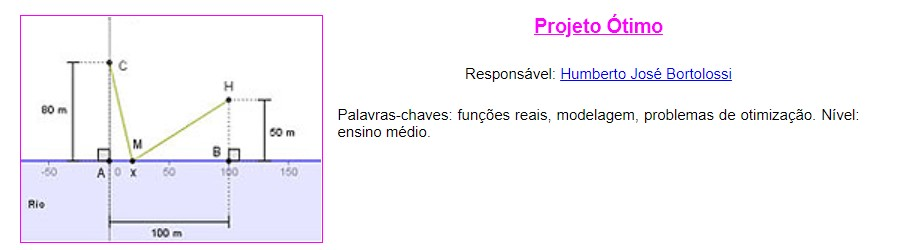
\includegraphics[width=\textwidth]{media/CDME-projeto-otimo.jpg}
    \caption{Thumbnail do Projeto Ótimo no site do CDME}
    \label{fig:projotimo}
\end{figure}

O Projeto Ótimo~(Figura \ref{fig:projotimo}) consiste de 21 módulos de problemas de otimização de uma variável acompanhados de construções GeoGebra, contextualizando a situação-problema, além de gráficos que relacionam as variáveis do domínio do problema com a imagem no contra-domínio. Os problemas exploram conceitos como domínio, imagem, gráfico de função, entre outros, estimulando conexões entre os aspectos algébrico, numérico, geométrico e verbal da função real. Para que o foco permaneça no processo de otimização propriamente dito, todas estas atividades possuem solução única e facilmente identificável como tal dentro do domínio.

Esses módulos vêm acompanhados de um documento com exercícios sugeridos que, caso o professor escolha usar, podem ser modificados para se adequarem aos alunos. Além disso, o professor pode utilizar as atividades de diversas maneiras: junto aos alunos em sala de aula; utilizando um projetor ou monitor; como atividade de casa após uma introdução em aula; em laboratório de informática da escola, deixando que os alunos discutam entre si e com o professor.
\\

A otimização --- tema do Projeto -- é, de maneira geral, o processo de maximizar ou minimizar o valor de uma função, através da uma escolha viável de suas variáveis segundo as condições impostas pela situação em que o problema se insere. Tais problemas são relevantes por serem extremamente comuns em praticamente qualquer área de atuação profissional: um empresário busca maximizar lucros; um engenheiro busca maior eficiência na produção; empresas de logística buscam maximizar a eficiência do roteamento de seus veículos. 
\\

Além de contextos humanos e profissionais, problemas de otimização também aparecem em contextos naturais: uma bolha de sabão é tal que a sua superfície é a mínima para um dado volume; a luz sempre percorre a distância que minimize a distância percorrida; e um objeto sempre tende ao equilíbrio em um ponto que minimize a sua energia potencial.

A grande relevância e recorrência deste tipo de problemas torna indispensável sua abordagem em sala de aula. Muitos dos alunos terão que \textit{otimizar} alguma tarefa ao longo de suas vidas, e a experiência de reconhecer domínios e contra-domínios, elaborar e modelar uma lei de função, aprender técnicas que facilitem suas resoluções, quando vista em sala de aula, pode acrescentar muito na formação escolar. 
\\

Cada módulo do Projeto Ótimo consiste de duas ou mais atividades. Uma atividade trata da otimização da situação apresentada, por exemplo, determinar a medida da base que maximiza a área de um triângulo, dado um perímetro fixo. Outra, aborda a modelagem geral de um problema, por exemplo, determinar a lei de formação de um triângulo de perímetro fixo, em função de sua base, seguindo o exemplo anterior. Essas atividade são acompanhados por uma simulação computacional gráfica da situação, que permite que o aluno interaja com o problema e tenha um melhor entendimento de suas particularidades e limitações. As situações também são acompanhadas de formulários de acompanhamento do aluno, que propõem reflexões adicionais sobre a estrutura do problema de otimização naquele contexto.

\begin{figure}[htb]
    \begin{subfigure}[b]{0.47\textwidth}
    \centering
    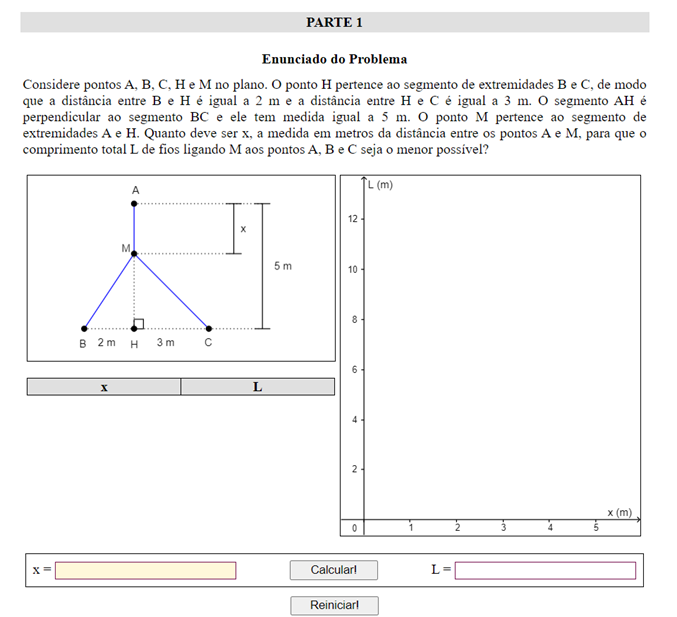
\includegraphics[width=\textwidth]{media/CDME-prob-geometrico-12.png}
    \caption{Exemplo de atividade do Projeto Ótimo sem nenhuma entrada/}
    \label{fig:otimo13-11}
    \end{subfigure}
    % 
    \hfill
    % 
    \begin{subfigure}[b]{0.47\textwidth}
    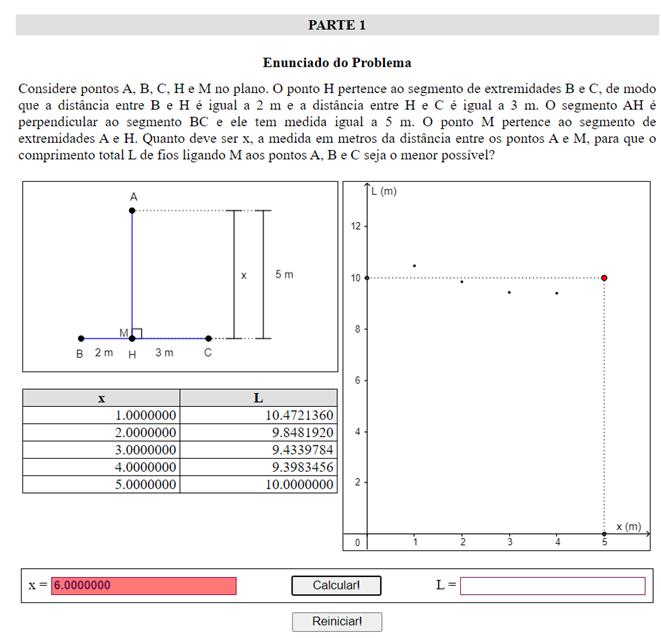
\includegraphics[width=\textwidth]{media/CDME-prob-geometrico-11.png}
    \caption{Exemplo de atividade do Projeto Ótimo após entradas válidas.}
    \label{fig:otimo13-12}
    \end{subfigure}
    \caption{Primeira parte do módulo 6: ``Um Problema Geométrico".}
    \label{fig:otimo13-1}
    
\end{figure}

\begin{figure}
\begin{subfigure}[b]{0.47\textwidth}
    \centering
    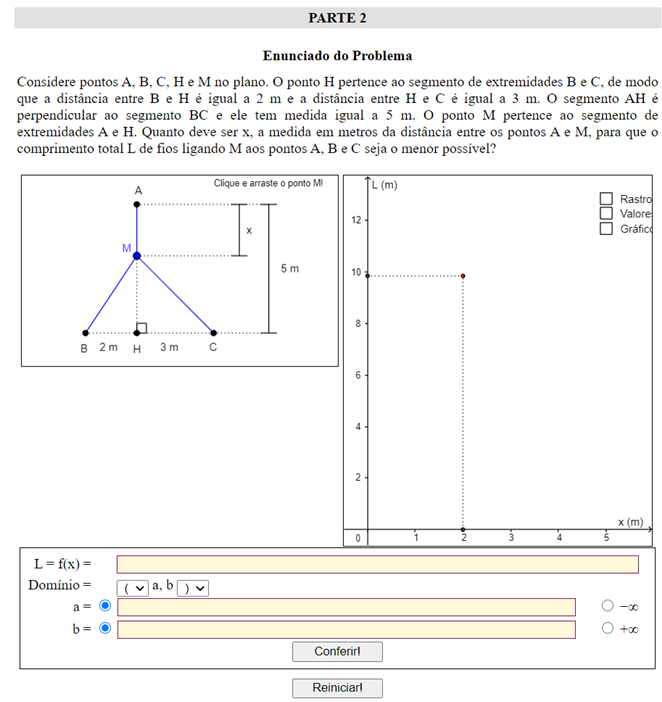
\includegraphics[width=8cm]{media/CDME-prob-geometrico-21.png}
    \caption{Atividade sem rastro nem linha do gráfico aparente}
\end{subfigure}
% 
\hfill
% 
\begin{subfigure}[b]{0.47\textwidth}
    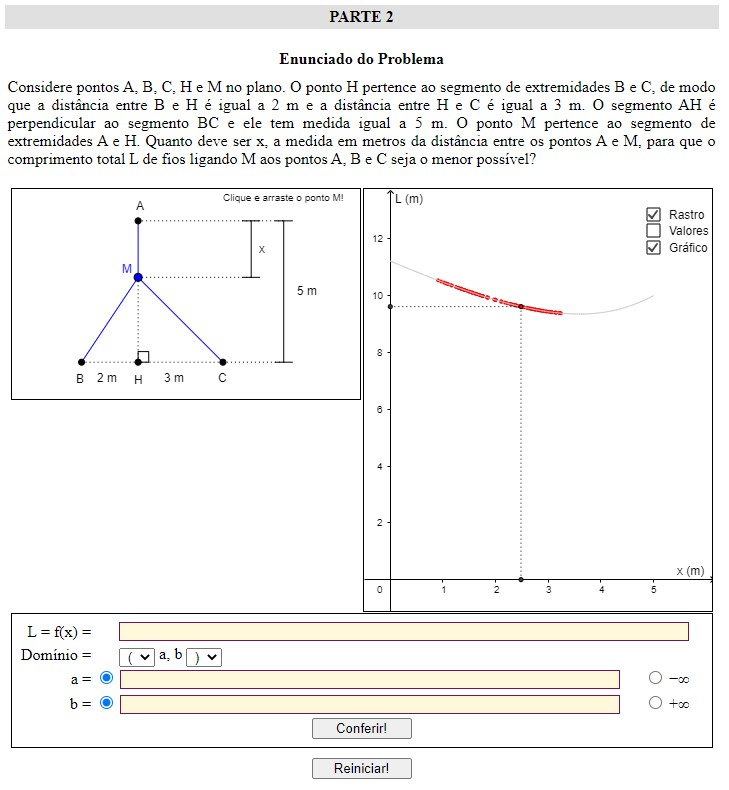
\includegraphics[width=8cm]{media/CDME-problema-geometric-grafico-rastro.jpg}
    \caption{Atividade com a linha do gráfico e alguns pontos do rastro aparentes aparente}
\end{subfigure}
    \caption{Segunda parte do módulo 6: ``Um Problema Geométrico"}
    \label{fig:otimo13-2}
\end{figure}

Um exemplo da estrutura citada no parágrafo anterior se encontra nas Figuras~\ref{fig:otimo13-1} e~\ref{fig:otimo13-2}. Na primeira parte o aluno deve buscar o valor da variável que otimiza o problema proposto. O valor da variável pode ser calculado ou estimado com o apoio das construções do GeoGebra, que exibem a situação-problema adaptada para o valor estimado da variável e a representação dessa estimativa no gráfico em uma tabela, como mostrado nas Figuras~\ref{fig:otimo13-11} e \ref{fig:otimo13-12}. Na segunda parte o aluno deve descrever a lei de formação da função e seu domínio, utilizando os conhecimentos que obteve na primeira etapa e uma nova construção GeoGebra, que permite interação clicando e arrastando nos pontos que representam a variável do domínio, ao mesmo tempo em que o gráfico é atualizado com o rastro deixado pelas variações. Também é possível ver diretamente o gráfico da função (Figura~\ref{fig:otimo13-2}).


Essa abordagem incentiva que o aluno entenda o problema e aprenda Matemática por meio de sua resolução. O entendimento de uma situação-problema traz benefícios como o de relacionar o pensar matemático com uma gama maior de contextos, estimular a capacidade do aluno de reconhecer ideias ou conceitos matemáticos, e ajuda a construir as relações entre as diversas ideias matemáticas que permeiam um dado problema~\cite{schroeder1989developing}.

Outra questão que vem à tona no Projeto Ótimo é a da representação matemática em contextos eletrônicos. A maior parte dos alunos está acostumada a representar os conceitos matemáticos através de símbolos --- $\sqrt{16}=4$, $2\pi\theta$, ou $2^3=8$, por exemplo --- que não são possíveis de escrever com teclados convencionais. Por isso, o aluno deve se familiarizar com a noção de que a representação de uma determinada operação ou conceito pode variar dependendo do contexto, e também se familiarizar com a maneira de escrevê-las da maneira que a programação do site entenda. Por exemplo, em contextos computacionais, é usual uma notação baseada no conceito de função, como em \texttt{sqrt()} para representa raiz quadrada. As operações aritméticas também possuem outras notações, como \^{} para representar potência, \texttt{*} para produto, etc. Também se faz necessário maior uso de parênteses para explicitar a precedência de operações, por exemplo \texttt{(x\^{}(25)+1)/(3\^{}2)} em vez de $\frac{x^{25}+1}{3^2}$.

\section{As atividades do Projeto Ótimo}

A seguir apresentaremos os 21 módulos do Projeto Ótimo, com seus respectivos enunciados e acompanhados de um pequeno comentário destacando pontos interessantes em cada um.

\begin{itemize}
    \item Módulo 1: ``O Problema da Cerca"
    
    ``Com 80 metros de cerca um fazendeiro deseja circundar uma região retangular junto a um rio para confinar alguns animais. O lado da região retangular junto a margem do rio não é cercado. Quanto deve ser x, a medida em metros da base da região retangular, para que a área cercada A seja a maior possível?”.
    
    É uma contextualização clássica de problema de otimização, que trabalha simultaneamente as noções de perímetro e área, evidenciando suas relações e diferenças com elementos muito comuns: cerca e área de terreno. Tem como pré-requisitos área e perímetro de retângulo, o Teorema de Pitágoras.
    
    
    \item Módulo 2: ``O Problema do Barbante: Quadrado e Círculo"
    
    ``Um fio de barbante de 10 metros de comprimento pode ser usado ou para construir um quadrado, ou para construir um círculo ou ele pode ser cortado em dois pedaços (não necessariamente de mesmo tamanho) de modo que um dos pedaços é usado para construir um quadrado e o outro pedaço é usado para construir um círculo. Quanto deve ser x, a medida em metros do pedaço do barbante usado para construir o quadrado, para que a soma S das áreas das figuras produzidas seja a maior possível? Quanto deve ser x, a medida em metros do pedaço do barbante usado para construir o quadrado, para que a soma S das áreas das figuras produzidas seja a menor possível?”.

    Trata da comparação entre a relação área-perímetro entre figuras geométricas diferentes --- círculo e quadrado, no caso. Tem como pré-requisitos área e perímetro de quadrados, área e perímetro de círculos, o Teorema de Pitágoras. 
    
    \item Módulo 3: ``O Problema do Barbante: Quadrado e Triângulo"
    
    % \begin{citacao}
    ``Um fio de barbante de 10 metros de comprimento pode ser usado ou para construir um quadrado, ou para construir um triângulo equilátero ou ele pode ser cortado em dois pedaços (não necessariamente de mesmo tamanho) de modo que um dos pedaços é usado para construir um quadrado e o outro pedaço é usado para construir um triângulo equilátero. Quanto deve ser x, a medida em metros do pedaço do barbante usado para construir o quadrado, para que a soma S das áreas das figuras produzidas seja a maior possível? Quanto deve ser x, a medida em metros do pedaço do barbante usado para construir o quadrado, para que a soma S das áreas das figuras produzidas seja a menor possível?”
    % \cite{cdme-pot}
    % \end{citacao}
    
    Módulo análogo ao anterior, agora com as figuras quadrado e triângulo equilátero. Serve como complemento e reforço para que o aluno entenda de onde vêm as proporções que maximizam a soma da área das figuras. Trata da comparação entre a relação área-perímetro entre figuras geométricas diferentes --- círculo e quadrado, no caso. Tem como pré-requisitos área e perímetro de quadrados, área e perímetro de triângulos equiláteros, o Teorema de Pitágoras. 
    
    \item Módulo 4: ``O Problema da Janela Normanda"
    
    ``Uma janela normanda tem o formato da justaposição de um semicírculo sobre um retângulo. Considerando as janelas normandas com perímetro igual a 9 m, quanto deve ser x, a medida em metros da base do retângulo que compõe a janela, para que a área A da janela seja a maior possível?”
    
    Aborda a relação que se apresenta entre o perímetro e a área de uma figura geométrica. Tem como pré-requisitos perímetro e área de retângulos, perímetro e área de semicírculos.
    
    \item Módulo 5: ``O Problema do Triângulo Isósceles"
    
    ``Considerando os triângulos isósceles com dois lados de medidas iguais a 3 m, quanto deve ser x, a medida em metros da base triângulo isósceles, para que a área A do triângulo seja a maior possível?”.
    
    Esse módulo traz a relação implícita entre ângulo e base de um triângulo com dois lados fixos, podendo ser usada para instigar o pensamento trigonométrico. tem como pré-requisitos área e perímetro de triângulos, o Teorema de Pitágoras.
    
    \item Módulo 6: ``Um Problema Geométrico"
    
     ``Considere pontos A, B, C, H e M no plano. O ponto H pertence ao segmento de extremidades B e C, de modo que a distância entre B e H é igual a 2 m e a distância entre H e C é igual a 3 m. O segmento AH é perpendicular ao segmento BC e ele tem medida igual a 5 m. O ponto M pertence ao segmento de extremidades A e H. Quanto deve ser x, a medida em metros da distância entre os pontos A e M, para que o comprimento total L de fios ligando M aos pontos A, B e C seja o menor possível?”
     
     É o primeiro módulo a não citar área, focando no teorema de Pitágoras e na relação cartesiana da distância entre um ponto fixo e um outro que varia em um eixo. Tem como pré-requisitos distância entre pontos no plano, o Teorema de Pitágoras.
    
    \item Módulo 7: ``O Problema do Caminho para A Horta"
    
    ``Um agricultor está em sua casa C situada a 80 metros da margem retilínea de um rio. Ele quer encher primeiro o seu regador de água em um ponto M na margem deste rio e, depois, se dirigir para sua horta H, situada a 50 metros da margem do rio. A distância entre os pés A e B das perpendiculares traçadas de C e H sobre a margem do rio é igual a 100 metros. Considere um sistema de coordenadas onde A = (0, 0), B = (100, 0), C = (0, 80), H = (100, 50) e M = (x, 0). Quanto deve ser x, a abscissa do ponto M sobre o eixo x, para que o comprimento d do trajeto casa (C), rio (M) e horta (H) seja o menor possível?”
    
    Pela primeira vez, o enunciando traz explicitamente a notação utilizada em planos cartesianos, e apresenta os primeiros conceitos relacionados à Geometria Analítica, instigando esse tipo de pensamento na cabeça do aluno sem necessariamente se aprofundar. O exercício do módulo em si é semelhante ao anterior, então valem os mesmos comentários, e os pré-requisitos são distância entre pontos no plano, o Teorema de Pitágoras.
    
    \item Módulo 8: ``O Problema da Distância entre Ponto e Reta"
    
    ``Dado um ponto A no plano cartesiano, quanto deve ser x para que a distância d entre A e M = (x, -2x + 4) (um ponto da reta y = -2x + 4) seja a menor possível?”
    
    O módulo traz, inserindo o conceito de função dentro do exercício de função, uma situação inteiramente composta de objetos Matemáticos. Dá, assim, oportunidade para o aluno desenvolver a sua capacidade de abstração, com o auxílio do gráfico. Tem como pré-requisito distância entre pontos no plano.
    
    \item Módulo 9: ``O Problema da Distância entre Ponto e Parábola"

    ``Dado um ponto A no plano cartesiano, quanto deve ser x para que a distância d entre A e M = (x, x$^2$) (um ponto da parábola y = x$^2$) seja a menor possível?”
    
    Assim como no módulo anterior, este propõe uma atividade contextualizada apenas com abstrações Matemáticas. Ao trabalhar com um objeto pouco frequente em problemas que envolvem distâncias, traz um questionamento mais aprofundado sobre a definição de distância de um ponto a um conjunto, no caso a parábola. Busca-se na atividade o ponto da parábola cuja distância ao ponto dado é mínima, isto é, o ponto que realiza a distância entre parábola e ponto.
    
    % caracterizar a distância de um ponto a um objeto, uma determinada curva a menor distância, ponto que pode ser resolvido intuitivamente e sem mais reflexões no módulo anterior. Tem como pré-requisito distância entre pontos no plano.
    
    \item Módulo 10: ``O Problema do Retângulo: Área e Perímetro"
    
    ``Considerando os retângulos de área igual a 3 m$^2$, quanto deve ser x, a medida em metros da base do retângulo, para que o perímetro y do retângulo seja o menor possível?”
    
    Aqui o projeto aborda novamente a relação de área e perímetro, dessa vez invertendo a relação proposta anteriormente, avaliando o perímetro em função da área. Tem como pré-requisitos área e perímetro de retângulo.
    
    \item Módulo 11: ``O Problema do Retângulo Inscrito num Círculo"
    
    ``Queremos encaixar (inscrever) dentro de um círculo um retângulo com a maior área possível. Se o círculo tem 3 metros de raio, quanto deve ser x, a medida em metros da base do retângulo, para que a área A do retângulo seja a maior possível?”
    
    Voltando a tratar o conceito de área em Geometria Plana, o módulo trabalha a ideia do problema de otimização com restrição com esse problema simples, oferecendo uma representação gráfica do problema. Tem como pré-requisitos área e perímetro de retângulos, o Teorema de Pitágoras.

    \item Módulo 12: ``O Problema do Triângulo Inscrito num Círculo"
    
    ``Queremos encaixar (inscrever) dentro de um círculo um triângulo isósceles com a maior área possível. Se o círculo tem 3 metros de raio, quanto deve ser x, a medida em metros da altura do triângulo, para que a área A do triângulo seja a maior possível?”
    
    Similarmente ao módulo anterior, explora a variação da área de um triângulo isósceles, com a restrição de estar inscrito em um círculo de raio fixo. Traz um exercício muito interessante envolvendo o teorema de Pitágoras, e tem com pré-requisitos área de triângulos, e o já mencionado Teorema de Pitágoras.
    
    \item Módulo 13: ``O Problema da Bobina do Transformador"
    
    ``Na construção de um transformador de corrente alternada, insere-se na bobina circular do transformador um núcleo de ferro cuja seção transversal tem o formato de uma cruz. É importante que esta seção transversal tenha a maior área possível. Se o raio da seção transversal circular da bobina mede 18 milímetros e se x representa a metade da medida, em milímetros, dos lados da cruz cujas extremidades estão sobre a seção circular, quanto deve ser x para que a área A da cruz seja a maior possível?"

    Esse módulo apresenta uma contextualização muito interessante vinda da engenharia, e começa a trabalhar com áreas não triviais. Nela o aluno deve quebrar a área da \textit{cruz} em áreas menores que ele consegue calcular, estimulando o pensamento de \textit{dividir para conquistar}, tão importante na matemática. Tem como pré-requisitos área de retângulos, o Teorema de Pitágoras.
    
    \item Módulo 14: ``O Problema da Caixa"
    
    ``Quadrados iguais são cortados dos cantos de uma folha de papelão retangular medindo 30 cm por 50 cm. As abas que sobram são então dobradas para cima de modo a formar uma caixa sem tampa. Quanto deve ser x, a medida em centímetros dos lados dos quadrados que são retirados da folha de papelão, para que o volume V da caixa seja o maior possível?”
    
    A partir desse módulo as atividades passam a tratar de geometria em três dimensões. O projeto inicia essa sequência com uma atividade que trata da relação entre área e volume em uma figura geométrica espacial. Tem como pré-requisitos área e perímetro de retângulos, volume de prismas retos quadrangulares.
    
    \item Módulo 15: ``O Problema da Caixa com Tampa"
    
    ``Um fabricante quer construir caixas com tampa a partir de uma folha de papelão retangular medindo 10 cm por 16 cm. Para construir a caixa, dois quadrados e dois retângulos são removidos dos cantos da folha de papelão. As abas que sobram são então dobradas para cima de modo a formar uma caixa com tampa. Quanto deve ser x, a medida em centímetros dos lados dos quadrados que são retirados da folha de papelão, para que o volume V da caixa seja o maior possível?”
    
    O módulo é muito similar ao anterior, com a diferença do formato da figura tratada. O fato de a caixa não ter tampa altera o corte feito, e assim muda a quantidade máxima de papelão que pode ser utilizada em uma situação dessa, excelente para promover o pensamento crítico. Tem como pré-requisitos área e perímetro de retângulos, volume de prismas retos quadrangulares.
    
    \item Módulo 16: ``O Problema do Bebedouro"
    
    ``Um bebedouro será construído na forma de um prisma reto cuja altura mede 7 m e cujas bases são trapézios. Cada trapézio tem base menor e laterais de medidas sempre iguais a 1 m. Se x representa a medida, em radianos, do ângulo entre uma lateral e uma altura de cada um dos dois trapézios congruentes usados na construção do bebedouro, quanto deve ser x para que a forma do bebedouro correspondente tenha o maior volume V possível?”
    
    Esse módulo se mostra interessante para abordar trigonometria, já que precisamos de uma maneira de relacionar os comprimentos das arestas com a variável sobre a qual temos algum controle: o ângulo. A questão do bebedouro se enchendo de água também traz a possibilidade de abordar o tema da semelhança entre sólidos. Tem como pré-requisitos área de triângulos, área de retângulos, trigonometria no triângulo retângulo, volume de prismas retos, o Teorema de Pitágoras.
    
    \item Módulo 17: ``O Problema da Embalagem Piramidal"
    
    ``Um fabricante quer construir uma embalagem no formato de uma pirâmide regular de base quadrada a partir de uma folha de papelão quadrada medindo 2 m por 2 m. Para construir a embalagem, triângulos isósceles são removidos das laterais da folha de papelão. As pontas que sobram são então dobradas para cima de modo a formar uma pirâmide regular de base quadrada. Quanto deve ser x, a metade da medida em metros da diagonal da base quadrada da pirâmide, para que o volume V da embalagem seja o maior possível?”
    
    Outro módulo que se estende sobre a relação entre área e volume de um sólido específico através da planificação, oferecendo uma estratégia interessante para a obtenção da planificação de uma pirâmide a partir de uma superfície quadrada. Tem como pré-requisitos elementos métricos do triângulo isósceles, elementos métricos do quadrado, volume de pirâmides regulares, o Teorema de Pitágoras.
    
    \item Módulo 18: ``O Problema do Cone"
    
    ``Um copo no formato cônico é feito com um disco circular de papel, de centro O, do qual foi retirado um setor circular AOM e os lados OA e OM foram unidos. Os lados OA e OM têm medida 7 cm. Quanto deve ser x, a medida em radianos do ângulo AOM, para que o volume V do copo seja o maior possível?”
    
    O último módulo explicitamente sobre relação entre área e volume, agora introduzindo um sólido não poliédrico, explora a relação da área lateral do cone como o seu volume. Tem como pré-requisitos perímetro de arcos de círculo, volume de cones circulares, o Teorema de Pitágoras.
    
    \item Módulo 19: ``O Problema do Cilindro Inscrito numa Esfera"
    
    ``Queremos encaixar (inscrever) dentro de uma esfera um cilindro circular reto com o maior volume possível. Se a esfera tem 3 metros de raio, quanto deve ser x, a medida em metros do raio da base do cilindro, para que o volume V do cilindro seja o maior possível?”
    
    Módulo análogo ao número 11, possibilita a discussão das simetrias de figuras geradas a partir de rotações de uma figura plana. Os pré-requisitos são volume de cilindros circulares, o Teorema de Pitágoras.
    
    \item Módulo 20: ``O Problema do Cone Inscrito numa Esfera"
    
    ``Queremos encaixar (inscrever) dentro de uma esfera um cone circular reto com o maior volume possível. Se a esfera tem 3 metros de raio, quanto deve ser x, a medida em metros da altura do cone, para que o volume V do cone seja o maior possível?”
    
    Um exercício parecido com o do Módulo 11, agora trabalhado em 3 dimensões. Possibilita essa discussão da Geometria Plana presente em seções de figuras tridimensionais. Tem como pré-requisitos volume de cones circulares, o Teorema de Pitágoras.
    
    \item Módulo 21: ``O Problema da Pirâmide Inscrita numa Esfera"
    
    ``Queremos encaixar (inscrever) dentro de uma esfera uma pirâmide regular de base quadrada com o maior volume possível. Se a esfera tem 3 metros de raio, quanto deve ser x, a medida em metros da altura da pirâmide, para que o volume V da pirâmide seja o maior possível?”
    
    O último módulo atualmente mistura a noção de poliedro --- a pirâmide inscrita --- com sólidos não poliédricos --- a esfera ---, que pode promover questionamentos interessantes se comparado com a atividade anterior. Quando pontos da pirâmide encostam na esfera, e como essa informação difere do caso do cone e o cilindro inscritos? Tem como pré-requisitos volume de pirâmides regulares, o Teorema de Pitágoras.
\end{itemize}

\begin{figure}
    \centering
    
    \begin{subfigure}{0.3\textwidth}
    \centering
    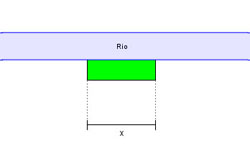
\includegraphics[width=.9\textwidth]{icones-modulos/pot-m-pce.jpg}
    \label{fig:pce-ic}
    \end{subfigure}
    \hfill
    \begin{subfigure}{0.3\textwidth}
    \centering
    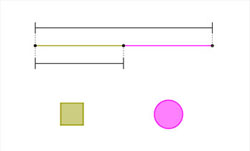
\includegraphics[width=.9\textwidth]{icones-modulos/pot-m-pbc.jpg}
    \label{fig:pbc-ic}
    \end{subfigure}
    \hfill
    \begin{subfigure}{0.3\textwidth}
    \centering
    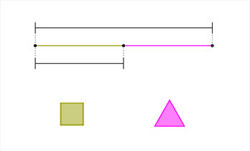
\includegraphics[width=.9\textwidth]{icones-modulos/pot-m-pbt.jpg}
    \label{fig:pbt-ic}
    \end{subfigure}
    
    \begin{subfigure}{0.3\textwidth}
    \centering
    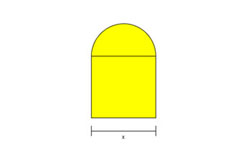
\includegraphics[width=.9\textwidth]{icones-modulos/pot-m-pjn.jpg}
    % \label{fig:pdc-ic}
    \end{subfigure}
    \hfill
    \begin{subfigure}{0.3\textwidth}
    \centering
    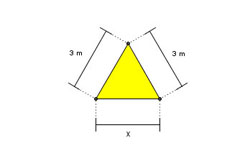
\includegraphics[width=.9\textwidth]{icones-modulos/pot-m-ptr.jpg}
    % \label{fig:pdc-ic}
    \end{subfigure}
    \hfill
    \begin{subfigure}{0.3\textwidth}
    \centering
    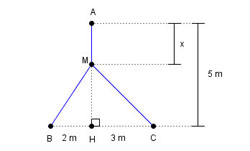
\includegraphics[width=.9\textwidth]{icones-modulos/pot-m-pge.jpg}
    \label{fig:pge-ic}
    \end{subfigure}
    
    \begin{subfigure}{0.3\textwidth}
    \centering
    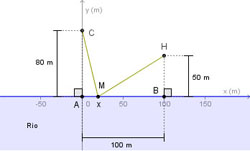
\includegraphics[width=.9\textwidth]{icones-modulos/pot-m-pch.jpg}
    % \label{fig:pch-ic}
    \end{subfigure}
    \hfill
    \begin{subfigure}{0.3\textwidth}
    \centering
    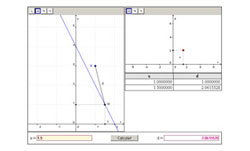
\includegraphics[width=.9\textwidth]{icones-modulos/pot-m-pre.jpg}
    \label{fig:pre-ic}
    \end{subfigure}
    \hfill
    \begin{subfigure}{0.3\textwidth}
    \centering
    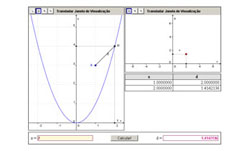
\includegraphics[width=.9\textwidth]{icones-modulos/pot-m-ppa.jpg}
    \label{fig:ppa-ic}
    \end{subfigure}
    
    \begin{subfigure}{0.3\textwidth}
    \centering
    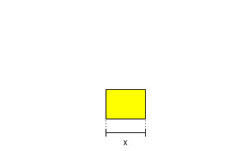
\includegraphics[width=.9\textwidth]{icones-modulos/pot-m-rap.jpg}
    \label{fig:rap-ic}
    \end{subfigure}
    \hfill
    \begin{subfigure}{0.3\textwidth}
    \centering
    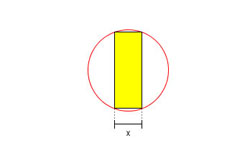
\includegraphics[width=.9\textwidth]{icones-modulos/pot-m-crt.jpg}
    \label{fig:crt-ic}
    \end{subfigure}
    \hfill
    \begin{subfigure}{0.3\textwidth}
    \centering
    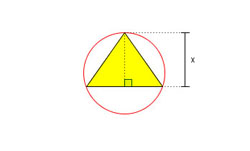
\includegraphics[width=.9\textwidth]{icones-modulos/pot-m-ctr.jpg}
    \label{fig:ctr-ic}
    \end{subfigure}
    
    \begin{subfigure}{0.3\textwidth}
    \centering
    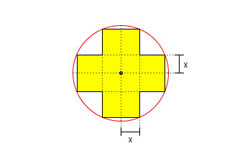
\includegraphics[width=.9\textwidth]{icones-modulos/pot-m-pbo.jpg}
    \label{fig:pbo-ic}
    \end{subfigure}
    \hfill
    \begin{subfigure}{0.3\textwidth}
    \centering
    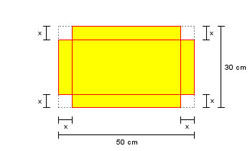
\includegraphics[width=.9\textwidth]{icones-modulos/pot-m-pdc.jpg}
    \label{fig:pdc-ic}
    \end{subfigure}
    \hfill
    \begin{subfigure}{0.3\textwidth}
    \centering
    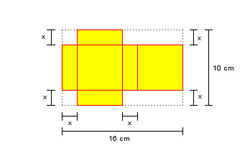
\includegraphics[width=.9\textwidth]{icones-modulos/pot-m-pct.jpg}
    \label{fig:pct-ic}
    \end{subfigure}
    
    
    \begin{subfigure}{0.3\textwidth}
    \centering
    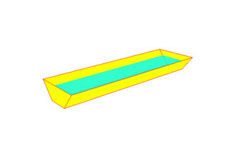
\includegraphics[width=.9\textwidth]{icones-modulos/pot-m-pbe.jpg}
    \label{fig:pbe-ic}
    \end{subfigure}
    \hfill
    \begin{subfigure}{0.3\textwidth}
    \centering
    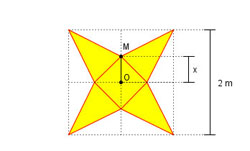
\includegraphics[width=.9\textwidth]{icones-modulos/pot-m-pep.jpg}
    \label{fig:pep-ic}
    \end{subfigure}
    \hfill
    \begin{subfigure}{0.3\textwidth}
    \centering
    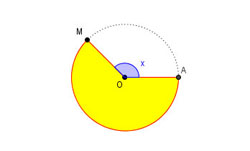
\includegraphics[width=.9\textwidth]{icones-modulos/pot-m-pco.jpg}
    \label{fig:pco-ic}
    \end{subfigure}
    
    \begin{subfigure}{0.3\textwidth}
    \centering
    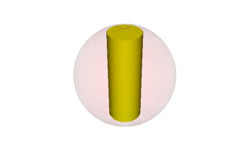
\includegraphics[width=.9\textwidth]{icones-modulos/pot-m-eci.jpg}
    \label{fig:eci-ic}
    \end{subfigure}
    \hfill
    \begin{subfigure}{0.3\textwidth}
    \centering
    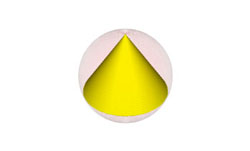
\includegraphics[width=.9\textwidth]{icones-modulos/pot-m-eco.jpg}
    \label{fig:eco-ic}
    \end{subfigure}
    \hfill
    \begin{subfigure}{0.3\textwidth}
    \centering
    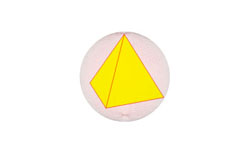
\includegraphics[width=.9\textwidth]{icones-modulos/pot-m-epi.jpg}
    \label{fig:epi-ic}
    \end{subfigure}
    
    \caption{Thumbnails dos módulos do Projeto Ótimo}
    \label{fig:icones-pot}
    
    
\end{figure}                %04
\chapter{Adaptação das atividades do Projeto Ótimo para HTML5}
\label{cap:partetecnica}

% Parte mais técnica:
% Detalhes mais técnicos sobre seu trabalho de readequação das atividades;
% Indicação para quem desejar continuar o trabalho de readequação das outras atividades do CDME.

% Tutorial/Roteiro para quem for fazer igual, com acesso ao código e/ou ferramentas que você utilizou.

% -> não tem mais suporte pra applets java nos navegadores hoje em dia
% -> o GeoGebra migrou a API deles pra javascript, mantendo todas as funções e etc
% -> O trabalho principal foi essa migração:
%     -> Usando o código ggbbase64 a gente consegue migrar de um pra outro relativamente fácil.
%     -> pra obter o código precisa abrir a construção em java e exportar como html
%     -> depois foi preciso escrever a estrutura da api nova: parâmetros, new GGBApplet, e applet.inject
% -> depois foi preciso adaptar a sintaxe pro modelo novo. applet.function() no lugar de document.getbyID('applet').function()


%Neste capítulo detalhamos o processo da substituição das construções em GeoGebra de applets java obsoletos por scripts, o novo padrão em vigência.


Neste capítulo detalhamos como atualizamos as atividades do Projeto Ótimo, que faziam uso extensivo de construções GeoGebra disponibilizadas como applets em Java, para versões destas atividades em que as construções foram disponibilizadas como scripts de JavaScript em HTML5. Como visto no capítulo~\ref{cap:historicoWeb}, applets em Java deixaram de ser suportados pelos navegadores atuais por motivos de segurança, e o JavaScript se tornou o novo padrão, adotado nativamente no HTML5. O novo padrão também traria novas funcionalidades além da maior segurança, como suporte para as construções em \textit{tablets} e telefones celulares, o que não era possível antes.
\\
Cada página do Projeto Ótimo continha pelo menos duas construções GeoGebra que deveriam ser substituídas. Para isso, foi necessário estudar a maneira que a implementação era feita, e buscar uma maneira de incorporá-los para as antigas construções. Para isso, utilizamos como consulta a \href{https://wiki.geogebra.org/en/Reference:GeoGebra_Apps_API}{página de referência da API do GeoGebra em JavaScript}.
\\

Abaixo, detalhamos passo a passo do trabalho feito para reimplementação das construções e atualização das atividades com a tecnologia atual. Embora as atividades do Projeto Ótimo já tenham sido todas convertidas, este processo poder ser útil para a conversão das demais páginas do Projeto CDME. Os exemplos abaixo seguirão o processo do módulo ``O Problema da Cerca", mas o processo é o mesmo para todas as atividades que não envolvem construções tridimensionais do GeoGebra.

Uma consequência do processo ser muito parecido para todos os módulos é que conseguimos automatizar o processo de conversão através de um script em Python, que tornaremos disponível em \url{https://github.com/fellipessanha/CDME-javascript/}.
\\

Vale ressaltar que todo o processo aqui descrito, apesar de partir de algum conhecimento prévio de programação de computadores, não exigiu qualquer experiência prévia com HTML, JavaScript, manutenção de sites, ou GeoGebra. Todo este conhecimento foi adquirido com a prática durante a própria resolução do problema aqui posto.

\section{Fazendo uma cópia local da página de cada atividade do Projeto Ótimo}

Utilizamos do fato de que as atividades do Projeto Ótimo são todas disponíveis para uso offline através de download para fazer a conversão. Cada módulo contém dois botões que possibilitam baixar todos os seus conteúdos, como mostra a figura~\ref{fig:serv02}. O arquivo baixado é um uma pasta comprimida(figura~\ref{fig:pdc-zip}) --- \texttt{pdc.zip}, no caso ---, e dentro da pasta \texttt{pdc-html}(figura~\ref{fig:pdc-html}) nós podemos encontrar todos os arquivos que vamos precisar modificar nesse processo da conversão.

\begin{figure}[hbt]
    \centering
    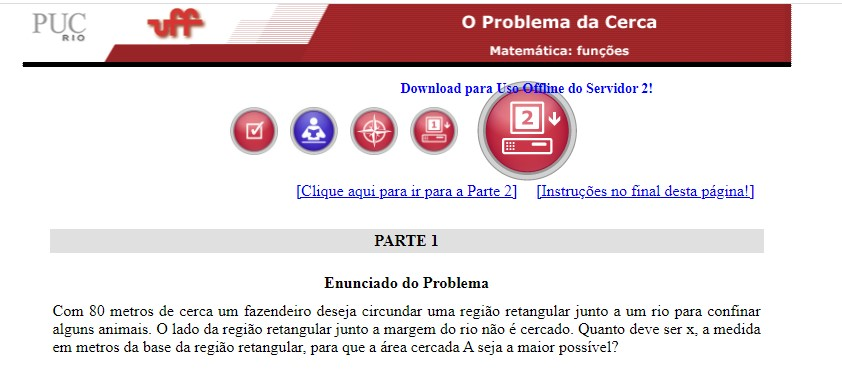
\includegraphics[width=\textwidth]{media/tec-print-servidor02.jpg}
    \caption{Botão ``Servidor 2", utilizado para baixar a cópia da atividade}
    \label{fig:serv02}
\end{figure}

\begin{figure}[hbt]
    \begin{subfigure}{0.5\textwidth}
    \centering
    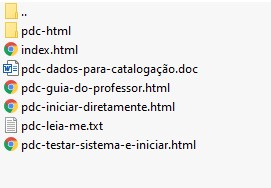
\includegraphics[width=.8\textwidth]{media/tec-pdc-zip.jpg}
    \caption{Todos os conteúdos do arquivo \texttt{pdc.zip}, com os conteúdos do módulo ``O Problema da Cerca"}
    \label{fig:pdc-zip}
    \end{subfigure}
    % 
    \hfill
    %  
    \begin{subfigure}{0.4\textwidth}
    \centering
    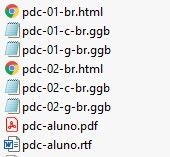
\includegraphics[width=.7\textwidth]{media/tec-pdc-html-alguns.jpg}
    \caption{Arquivos importantes dentro da pasta \texttt{pdc-html}, dentro da cópia do módulo ``O Problema da Cerca".}
    \label{fig:pdc-html}
    \end{subfigure}
    \caption{Imagens dos conteúdos do arquivo baixado do CDME.}
\end{figure}

\section{Obtendo o código de identificação de cada construção GeoGebra}

Ao longo do processo, descobrimos que o método que utilizaríamos para incorporar as construções em suas respectivas páginas exigia termos um código de identificação de cada atividade, que não estava presente na versão anterior do Projeto. Este código, é uma transcrição em formato \texttt{ggbBase64}\footnote{Um código em formato ggbBase64 é um texto composto de até 64 caracteres diferentes (base 64), que contém todas as informações de uma construção de maneira que a API do GeoGebra consiga decodificar.} das construções. Descobrimos que os códigos em ggbBase64 das construções podem ser gerados através do programa GeoGebra em sua versão ``3.2.46.11", exportando os arquivos como arquivos HTML, como mostrado na Figura~\ref{get-ggbBase64}.

\begin{figure}[htb]
    \centering
    
    \begin{subfigure}{\textwidth}
    \centering
    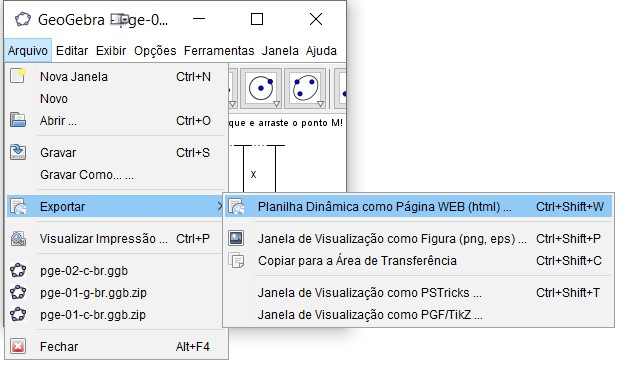
\includegraphics[width=0.7\textwidth]{media/tec-get-ggbBase64-01}
    \caption{Botão que abre a janela de exportação para html. Também pode ser usado o atalho Ctrl+Shift+W}
    \label{fig:getggb1}
    \end{subfigure}
    
    \begin{subfigure}{\textwidth}
    \centering
    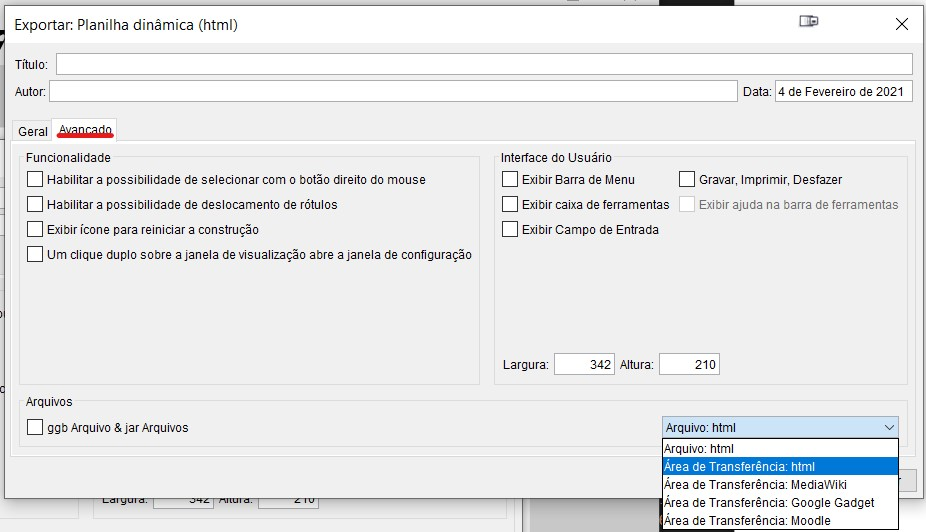
\includegraphics[width=0.9\textwidth]{media/tec-get-ggbBase64-02}
    \caption{A Janela de exportação do arquivo GeoGebra para html. Ambas as opções HTML te dão o mesmo texto, mas uma salva o arquivo no disco, e a outra simplesmente copia o texto para a área de transferência, onde pode ser colada em algum outro arquivo.}
    \label{fig:getggb2}
    \end{subfigure}
    \caption{Procedimento para obtenção do código de identificação ggbBase64 pelo programa \texttt{geogebra.jar}.}
    \label{get-ggbBase64}
\end{figure}

\begin{verbatim}
<applet name="ggbApplet" code="geogebra.GeoGebraApplet"
archive="geogebra.jar"
codebase="http://www.geogebra.org/webstart/3.2/unsigned/"
width="342" height="200" mayscript="true">
<param name="ggbBase64" value="{codigo-de-identificação}"/>
\end{verbatim}

Será gerado um único arquivo com extensão html. Este arquivo deve ser aberto com um editor de texto, e deve-se buscar o código de identificação dentro da tag como abaixo: 

O valor da o atributo \texttt{codigo-de-identificação} é a codificação em ggbBase64 da construção. Este valor é um texto muito longo. Outros parâmetros que serão úteis posteriormente são \texttt{width} e \texttt{height}, que nos informam, respectivamente, a largura e a altura, em pixels, da construção.

\section{Atualizando a página de atividade}

Com a identificação em mãos, a incorporação das construções se torna possível, introduzindo das seguintes linhas de código no lugar da antiga tag \texttt{<applet>}:

Abrindo a página da atividade (no nosso caso, a página ...) com um editor de texto, todo o conteúdo entre as tag \texttt{<applet>} e \texttt{</applet>}, incluindo estas tags, deve ser substituído pelas linhas abaixo:


\begin{verbatim}
    <script>
    var params_construct = {
          "id": "ggbApplet",
          "width":354,
          "height":214,
          "showMenuBar":false,
          "showAlgebraInput":false,
          "showToolBar":false,
          "showToolBarHelp":false,
          "showResetIcon":false,
          "enableLabelDrags":false,
          "enableShiftDragZoom":false,
          "enableRightClick":false,
          "errorDialogsActive":false,
          "useBrowserForJS":false,
          "ggbBase64": {codigo-de-identificação-obtido-na-seção-anterior}
          };
    params_construct.appletOnLoad = function(api) {
        /* ações necessárias mediante carregamento da construção */ };
    var construct_id = new GGBApplet("5.0", params_construc);
    window.addEventListener("load", function(){
        construct_id.inject("construct_id_container", "auto")});
    </script>
\end{verbatim}

O valor do campo \texttt{ggbBase64} de uma construção é o obtido a partir do seu respectivo arquivo .ggb, como descrito na seção anterior. Os valores de \texttt{width} e \texttt{height} podem ser os que foram obtidos naquela seção também, mas podem ser qualquer largura e altura convenientes.

As ações necessárias mediante carregamento já estavam bem definidas no código antigo, e aqui só foi necessário atualizar o método pelos quais eram chamadas.

\section{Adaptando o código para a API atual}

Após essas mudanças, as construções já devem estar operacionais na página, mas a programação que faz a comunicação dos applets com os botões e campos HTML ainda não deve estar funcionando, pois ainda estão na sintaxe utilizada pelos applets. Para sanar esse problema, temos que reescrever a maneira que as funções são chamadas no código.
\\

No modelo antigo, uma função \texttt{nome\_func}, de parâmetros \texttt{parametros\_func}  que interagia com o applet Java de uma construção \texttt{id\_construct} era chamada da seguinte maneira:

\begin{verbatim}
  document.getElementById("id_construct").nome_func(parametros_func);
\end{verbatim}

No GeoGebra para JavaScript, a mesma função, com os mesmos parâmetros e que interage com a mesma construção deve ser chamada da seguinte maneira:

\begin{verbatim}
    id_construct.nome_func(parametros_func);
\end{verbatim}

Essas mudanças podem ser feitas em qualquer editor de texto. Há alguns, como o Visual Studio Code, que possuem ferramentas para substituir todas as repetições de uma determinada sequência de caracteres\footnote{Conhecidas como \textit{strings} no mundo da informática.}

\section{Automatizando a atualização}

Todo o processo foi automatizado através de um \textit{script} em Python, disponível em repositório no GitHub, acessível em \url{https://github.com/fellipessanha/CDME-javascript/}, que fez as substituições como explicadas acima em todas as páginas.

O \textit{script} retira informações úteis --- como código de identificação ggbBase64, e opções como tornar a barra de menus inacessível --- de páginas HTML localizadas em uma pasta dentro do repositório, cria um código JavaScript que possibilita a inserção da construção na página da atividade, insere a atividade no lugar correto, e salva o código da página nova, com a codificação correta, em um arquivo separado, para evitar sobrescrever o código original.
\\

Para executar o código, basta executar o arquivo \texttt{conversion.py}, disponível no \href{https://github.com/fellipessanha/CDME-javascript/}{repositório}, com o Python, dentro do diretório da pasta que contém tanto as páginas que cujas construções devem ser convertidas, quanto a pasta com os respectivos códigos html das construções. No Windows, basta abrir o Prompt de Comando, navegar até a sua pasta destino --- \texttt{cd <pasta-destino>} --- e executar o comando ``\texttt{python conversion.py}". O programa atualiza com uma mensagem de texto para cada construção corretamente convertida.


\section{Módulos com construções tridimensionais}

Outro problema que se apresentou a nós foi o das construções tridimensionais, antes feitas com o software de visualização de figuras 3D JavaView. Ao contrário do GeoGebra, os desenvolvedores dessa biblioteca não disponibilizam nenhum tipo de suporte que nos permita converter as construções para implementação em HTML5, o que significa que tivemos que refazer todo o trabalho de visualização de figuras tridimensionais que correspondessem às situações propostas e, além de passarem no teste do arrastamento~\cite{de2020fases}, se comportassem como as já previamente utilizadas, além do esforço de formatação para encaixar o novo software no lugar do antigo..
\\

Escolhemos como ferramenta para solucionar o problema supracitado o próprio GeoGebra, que hoje em dia conta com suporte a janelas tridimensionais. Essa escolha tem a vantagem de padronizar todos os softwares do projeto facilitando qualquer tipo de manutenção futura no site, já que todas as construções terão funcionamentos similares.

Formatar as construções para que se encaixassem nos mesmos locais pré-definidos para os applets anteriores se mostrou a tarefa mais trabalhosa, visto que as construções eram muito diferentes entre si. A formatação foi feita ajeitando as figuras aos poucos, e testando o resultado na página do respectivo módulo.
\\

Além da formatação, foi necessário rodar alguns durante a inicialização da construção para garantir que o mouse se comportase como esperado, rotacionando a construção em torno de um eixo específico. O código utilizado é como o especificado abaixo:
\\

\begin{verbatim}
    var parameters3d ={
        "appletOnLoad":function(api){api.setMode(540);},
        /* variáveis necessárias para a construção */
    }
\end{verbatim}


Os conteúdos do parâmetro ``\texttt{appletOnLoad}" são os métodos executados pelo GeoGebra em sua inicialização, e o método especificado --- ``\texttt{api.setMode(540);}" --- serve para modificar a função do mouse na construção para alterar o ângulo da perspectiva da construção, ao invés da função original de interação com a figura.

% </script>
% <div id="lspApplet_container"></div>
% </td>
% <td align="center" bgcolor="#FFFFFF">
% <script>
%   var parameters = {
%   "id": "ggbApplet",
%   "width":354,
%   "height":214,
%   "showMenuBar":false,
%   "showAlgebraInput":false,
%   "showToolBar":false,
%   "customToolBar":"0 | 1 501 5 19 , 67 | 2 15 45 18 , 7 37 | 514 3 9 , 13 44 , 47 | 16 51 | 551 550 11 ,  20 22 21 23 , 55 56 57 , 12 | 69 | 510 511 , 512 513 | 533 531 , 534 532 , 522 523 , 537 536 , 535 , 538 | 521 520 | 36 , 38 49 560 | 571 30 29 570 31 33 | 17 | 540 40 41 42 , 27 28 35 , 6 , 502",
%   "showToolBarHelp":false,
%   "showResetIcon":false,
%   "enableLabelDrags":false,
%   "enableShiftDragZoom":false,
%   "enableRightClick":false,
%   "errorDialogsActive":false,
%   "useBrowserForJS":false,
%   "allowStyleBar":false,
%   "preventFocus":false,
%   "showZoomButtons":true,
%   "capturingThreshold":3,
%   // add code here to run when the applet starts
%   "appletOnLoad":function(api){ /* api.evalCommand('Segment((1,2),(3,4))');*/ },
%   "showFullscreenButton":false,
%   "scale":1,
%   "disableAutoScale":false,
%   "allowUpscale":false,
%   "clickToLoad":false,
%   "appName":"classic",
%   "showSuggestionButtons":false,
%   "buttonRounding":0.7,
%   "buttonShadows":false,
%   "language":"pt",
%   // use this instead of ggbBase64 to load a material from geogebra.org
%   // "material_id":"RHYH3UQ8",
%   // use this instead of ggbBase64 to load a .ggb file
%   // "filename":"myfile.ggb",
%   "ggbBase64": 'codigo=enorme'
%   };
%   // is3D=is 3D applet using 3D view, AV=Algebra View, SV=Spreadsheet View, CV=CAS View, EV2=Graphics View 2, CP=Construction Protocol, PC=Probability Calculator DA=Data Analysis, FI=Function Inspector, macro=Macros
%   var views = {'is3D': 1,'AV': 0,'SV': 0,'CV': 0,'EV2': 0,'CP': 0,'PC': 0,'DA': 0,'FI': 0,'macro': 0};
%   var applet = new GGBApplet(parameters, '5.0', views);
%   window.onload = function() {applet.inject('ggbApplet')};
%   applet.setPreviewImage('data:image/gif;base64,R0lGODlhAQABAAAAADs=','https://www.geogebra.org/images/GeoGebra_loading.png','https://www.geogebra.org/images/applet_play.png');
% //   ggbApplet.registerObjectUpdateListener('variavelX')
%   </script>        %05
\chapter{Conclusão}
\label{cap:conclusao}
% -> uso da tecnologia bem-feito pelos autores do cdme, vim pra atualizar a tecnologia
% -> tecnologia precisa de atualização senão dá ruim
% -> não cair na ladainha de ver o computador como uma televisão
% -> trabalho legal de uso da tecnologia correu o risco de se perder, e ainda tem coisa pra consertar lá no cdme

% seção ensino

Como vimos nos capítulos~\ref{cap:recComputacionais}~e~\ref{cap:CDME}, o Projeto Ótimo --- e também o CDME, como um todo --- faz um uso exemplar das tecnologias digitais no Ensino da Matemática, utilizando de seu alto dinamismo e capacidade de modelagem em problemas de otimização, com o objetivo de estimular as conexões entre os aspectos algébrico, numérico, geométrico e verbal de uma função real, trabalhando a capacidade de modelagem matemática, tão importantes na formação matemática moderna.

Respeitando a função do computador enquanto máquina de modelagem, o trabalho abre portas a propostas modernas em Educação Matemática, que privilegiam não mais os conteúdos em si, mas sim o \textit{fazer matemático}, que envolve o processo de heurístico que leva às respostas em um raciocínio matemático próprio.
\\

Dessa forma, a atualização do Projeto Ótimo aqui feito tem o potencial de impactar o aprendizado de alunos de todo o Brasil, por proporcionar uma abordagem diferente para o ensino de problemas de otimização.
\\

% seção extensão:
Tratamos, durante todo o trabalho, da relação entre as tecnologias e seus usos, de como a perda de popularidade de um determinado uso de tecnologia pode acarretar o desuso de uma tecnologia, ou como o avanço na tecnologia pode, eventualmente, criar incompatibilidades que impossibilitem usos anteriores, ainda que relevantes.
% {\color{red}[juntar com parágrafo anterior]}
O caso do Projeto Ótimo se encaixa neste último caso, e infelizmente correu o risco de se perder na incessável marcha da tecnologia moderna. Porém, com algum conhecimento de programação e um trabalho de pesquisa, foi possível recuperar esse conteúdo e disponibilizá-lo novamente para o grande público, mantendo assim o trabalho universitário de qualidade feito para a sociedade nesse projeto de extensão.
\\

% seção pesquisa

O capítulo~\ref{cap:recComputacionais} expõe uma visão sobre tecnologias, sua evolução, faz um apanhado geral sobre a visão do uso de tecnologias no ensino de Matemática, e avalia como essa relação evoluiu com o tempo, em diferentes fases. Mostra que a literatura aponta para um caminho diferente do seguido atualmente por grande parte das escolas brasileiras,propondo que a ênfase do ensino seja mais voltada para um fazer matemático, em que o caminho que leva às respostas é pensado como parte do processo de ensino.
\\

Apresentamos no capítulo~\ref{cap:CDME} um apanhado geral da história do CDME e do Projeto Ótimo, e investigamos mais a fundo a abordagem do Projeto sobre problemas de otimização e os outros pontos importantes Procuramos explicitar a importância de se trabalhar com situações-problema no ensino de Matemática e usar isso como meio para ensinar os conceitos importantes, além da importância de ter um conhecimento básico da linguagem matemática entendida pelo computador no futuro dos alunos, que já vivem em um mundo permeado por TICs.
\\

% {\color{blue}
Vimos nos capítulos~\ref{cap:historicoWeb}~e~\ref{cap:partetecnica} que a manutenção de recursos educacionais online deve ser um trabalho ativo, e mostramos nesse trabalho que, mesmo com experiência limitada com as tecnologias em questão, é possível realizar essas manutenções, e que alguns conhecimentos a mais de programação de propósito geral conseguem inclusive automatizar alguns processos dessa tarefa.
\\

% seção costura
Por fim, o trabalho buscou se basear no tripé universitário ensino-pesquisa-extensão: por se propôr a fazer um trabalho que impactasse diretamente a educação matemática, através do Projeto Ótimo; por fazer um levantamento do histórico do projeto, do uso de tecnologia na educação, e do histórico do uso das tecnologias, sejam elas da informação ou não; e por promover um trabalho prático de revitalização de uma página que contribui de fato com a sociedade, ao promover o ensino de problemas de otimização de uma maneira tão rica.
% }

% -> Assim como a evolução da tecnologia e a evolução do uso da tecnologia se influenciam (você falou sobre isso),  as obsolescências também podem se influenciar. Quando um problema deixa de ser um problema, as tecnologias que eram utilizadas na solução podem cair em desuso, se não fossem utilizadas para mais problemas (um exemplo disso seria interessante). Da mesma forma, uma tecnologia obsoleta pode comprometer um uso de tecnologia, mesmo que o problema ainda seja relevante.

% -> O Projeto Ótimo, cai no segundo caso. Um uso excelente da tecnologia, tratando muito bem de um problema ainda relevante, mas que perdeu a funcionalidade porque a tecnologia caiu em obsolescência. Isso, inclusive, dá muita força e justificativa ao seu trabalho.

% -> Pode falar que o seu TCC buscou fazer um apanhado de visões sobre tecnologia e seu uso no Ensino de Matemática, uma vez que o que o Projeto Ótimo e tudo o que ocorreu com ele é um ótimo (trocadilho aí) exemplo de como tecnologia e uso se misturam. No caso, o primeiro acabou limitando o segundo.

% -> Lá naquele capítulo sobre uso de TICs no Ensino, você poderia incluir um parágrafo dizendo que quem se utiliza de uma tecnologia deve levar em conta, na hora de a utilizar, que ela não é eterna e pode eventualmente cair em desuso. Temos vários exemplos disso, desde artefatos concretos que se baseiam em material que não são mais encontrados no mercado, como recursos digitais baseados em frameworks caducos.

% \printbibliography
\bibliography{references.bib}

\end{document}
